% +------ AUTORIA DO PROJETO ------+
%	Autor: António César Vieira da Cruz Júnior
%	Email: antoniojr@icomp.ufam.edu.br
%	Período: 2018/1
% +------ TEMPLATE FONTE TCC ------+
% 	Autor: Arllem Farias, 2017.
% 	Email: arllemfarias@ufam.edu.br
%   Revisor: João Victor Lima Lopes
%   Email: jvllopess@gmail.com
% +--------------------------------+

% Ítens como: Ficha Catalográfica, Folha de Aprovação Assinada e Lombada, devem ser adicionadas posteriormente
% e descomentar as linhas que as adicionam (Linhas 132,134 e 135).

% Classe do documento --> \documentclass[OPÇÕES]{CLASSE}
\documentclass[
			   a4paper, % Tipo de papel 
			   oneside, % Impressão em apenas um lado da folha
			   12pt     % Tamanho da fonte
			   ]{book}  % Classe do documento

% Pacotes --> \usepackage[OPÇÕES]{PACOTE}
\usepackage[utf8]{inputenc} % Codificação do documento (conversão automática dos acentos) 
\usepackage[brazil]{babel}  % Traduz palavras chaves para o PT-BR (ex.: abstract->resumo)
\usepackage{indentfirst}    % Indenta o primeiro parágrafo de cada seção
\usepackage{setspace}		% Possibilita a alteração do espaçamento entre linhas
\usepackage{graphicx}       % Possibilita a inserção de figuras
\usepackage{subcaption}     % Possibilita a inserção de subfiguras
\usepackage{pdfpages}       % Possibilita a inserção de páginas em pdf
\usepackage{amsmath}        % Inclui funções adicionais no ambiente matemático \eqref{•} \dfrac{•}{•}
\usepackage{amssymb} 		% Símbolos adicionais no documento \mathbb{R}
\usepackage{mathrsfs}       % Símbolos da transformadas de Laplace e Fourier \mathscr{•}
\usepackage{float}			% Possibila posicionar tabelas e figuras em uma posição específica [H]
\usepackage[numbers]{natbib}% Inclui mais possibilidades de citações \citep{•}
\usepackage{fancyhdr}       % Possibilita a alteração de cabeçalho e rodapé
\usepackage{longtable}      % Possiblita a quebra de tableas em duas páginas
\usepackage{multirow}		% Possibilita multiplas linhas em tabelas
\usepackage{array}			% Possibilita o uso do comando \newcolumntype{•}[•]
\usepackage{pdflscape}      % Possibilita a inserção de páginas em modo paisagem
\usepackage{listings}		% Possibilita inserir códigos fontes (C++, Java, ...)
\usepackage{slashbox}       % Adiciona o comando \backslashbox{•}{•} usado em tabelas
\usepackage{arydshln}       % Possibilita inserir linhas pontilhadas em tabelas 
\usepackage{copyrightbox}
\usepackage{epigraph}
\usepackage[framed,numbered]{matlab-prettifier}

%\usepackage[inline]{showlabels} % Mostra os labels das equações
%\usepackage[notcite,notref]{showkeys} % Mostra todo os labels
%\usepackage{lipsum} % preenchimento automático de textos

% Modifica os itens do sumário
\usepackage[nottoc,
			notlof,
			notlot]{tocbibind}

% Configura as margens das páginas
\usepackage[top    = 3cm,
			bottom = 2cm,
			left   = 3cm,
			right  = 2cm]{geometry}

% Possibilita hiperlinks no texto
\usepackage[pdftex,
			%backref,
			linktocpage = false,
			colorlinks  = true,
			linkcolor   = blue,
			anchorcolor = blue,
			citecolor   = blue,
			urlcolor    = blue]{hyperref}

% Comandos auxiliares --> \nomecomando{COMANDO}{•}
\newcolumntype{C}[1]{>{\centering\let\newline\\\arraybackslash\hspace{0pt}}m{#1}} % Tabelas: {|C{2cm}|C{5cm}|}
\newcolumntype{L}[1]{>{\let\newline\\\arraybackslash\hspace{0pt}}m{#1}} % Tabelas: {|L{2cm}|L{5cm}|}
\newcommand*{\doi}[1]{DOI: \href{http://dx.doi.org/#1}{#1}} % Usado nas referencias

\setcounter{secnumdepth}{3} % Inclui a numeração de \subsubsection{•} no documento
\setcounter{tocdepth}{3}    % Inclui a \subsubsection{•} no sumário
\setstretch{1.5}			% Configura o espaçamento entre linhas \usepackage{setspace}

\pagestyle{fancy} 			% Configura a página para incluir o cabeçalho e rodapé
\lhead{{\footnotesize\leftmark}} % Cabeçalho esquerdo
\chead{}				         % Cabeçalho central
\rhead{\thepage}				 % Cabeçalho direito
\fancyfoot{}					 % Rodapé vazio

% Definição de novas cores
\definecolor{mygreen}{RGB}{0, 115, 0}
\definecolor{mylilas}{RGB}{170,55,240}


% Novos comandos --> \newcommand{COMANDO}{DEFINIÇÃO}
\newcommand{\instituicao}{
				UNIVERSIDADE FEDERAL DO AMAZONAS\\
				FACULDADE DE TECNOLOGIA\\
				ENGENHARIA DA COMPUTAÇÃO}
\newcommand{\titulo}{
				SISTEMA DE DETECÇÃO DE FREQUÊNCIA FUNDAMENTAL PARA MÚSICA}
\newcommand{\apresentacao}{
				Monografia apresentada à Coordenação do Curso
				de Engenharia da Computação da Universidade Federal
				do Amazonas, como parte dos requisitos necessários
				à obtenção do título de Engenheiro de Computação.}
\newcommand{\autor}{
				ANTÓNIO CÉSAR VIEIRA DA CRUZ JÚNIOR}
\newcommand{\local}{
				MANAUS-AM\\2018}
\newcommand{\orientador}{
				WALDIR SABINO DA SILVA JÚNIOR}
			

% Others commands
\newcommand{\rreg}{$\textsuperscript{\textregistered}$\space}
\renewcommand{\lstlistingname}{Algorítmo}

\usepackage{algpseudocode,algorithm}
% Declaracoes em Português
\algrenewcommand\algorithmicend{\textbf{fim}}
\algrenewcommand\algorithmicdo{\textbf{faça}}
\algrenewcommand\algorithmicwhile{\textbf{enquanto}}
\algrenewcommand\algorithmicfor{\textbf{para}}
\algrenewcommand\algorithmicif{\textbf{se}}
\algrenewcommand\algorithmicthen{\textbf{então}}
\algrenewcommand\algorithmicelse{\textbf{senão}}
\algrenewcommand\algorithmicreturn{\textbf{devolve}}
\algrenewcommand\algorithmicfunction{\textbf{função}}

% Rearranja os finais de cada estrutura
\algrenewtext{EndWhile}{\algorithmicend\ \algorithmicwhile}
\algrenewtext{EndFor}{\algorithmicend\ \algorithmicfor}
\algrenewtext{EndIf}{\algorithmicend\ \algorithmicif}
\algrenewtext{EndFunction}{\algorithmicend\ \algorithmicfunction}

% O comando For, a seguir, retorna 'para #1 -- #2 até #3 faça'
\algnewcommand\algorithmicto{\textbf{até}}
\algrenewtext{For}[3]%
{\algorithmicfor\ #1 $\gets$ #2 \algorithmicto\ #3 \algorithmicdo}

%-----------------------------------------------------
%\usepackage{ulem}
%\newcommand{\commentib}[1]{{\color{red} [IB: #1]}}
%\newcommand{\corrigir}[1]{{\color{violet}\uwave{#1}}}
%-----------------------------------------------------

\begin{document}

\begin{titlepage}

\begin{center}

\begin{figure}[t]
	\centering
	\includegraphics[scale=0.7]{pasta1_figuras/logo_ufam.eps}
\end{figure}

\textbf {\instituicao}

\vfill
\textbf{\Large \titulo}

\vfill
\textbf{\autor}

\vfill
\textbf{\local}

\end{center}

\end{titlepage}

%\begin{titlepage}
	
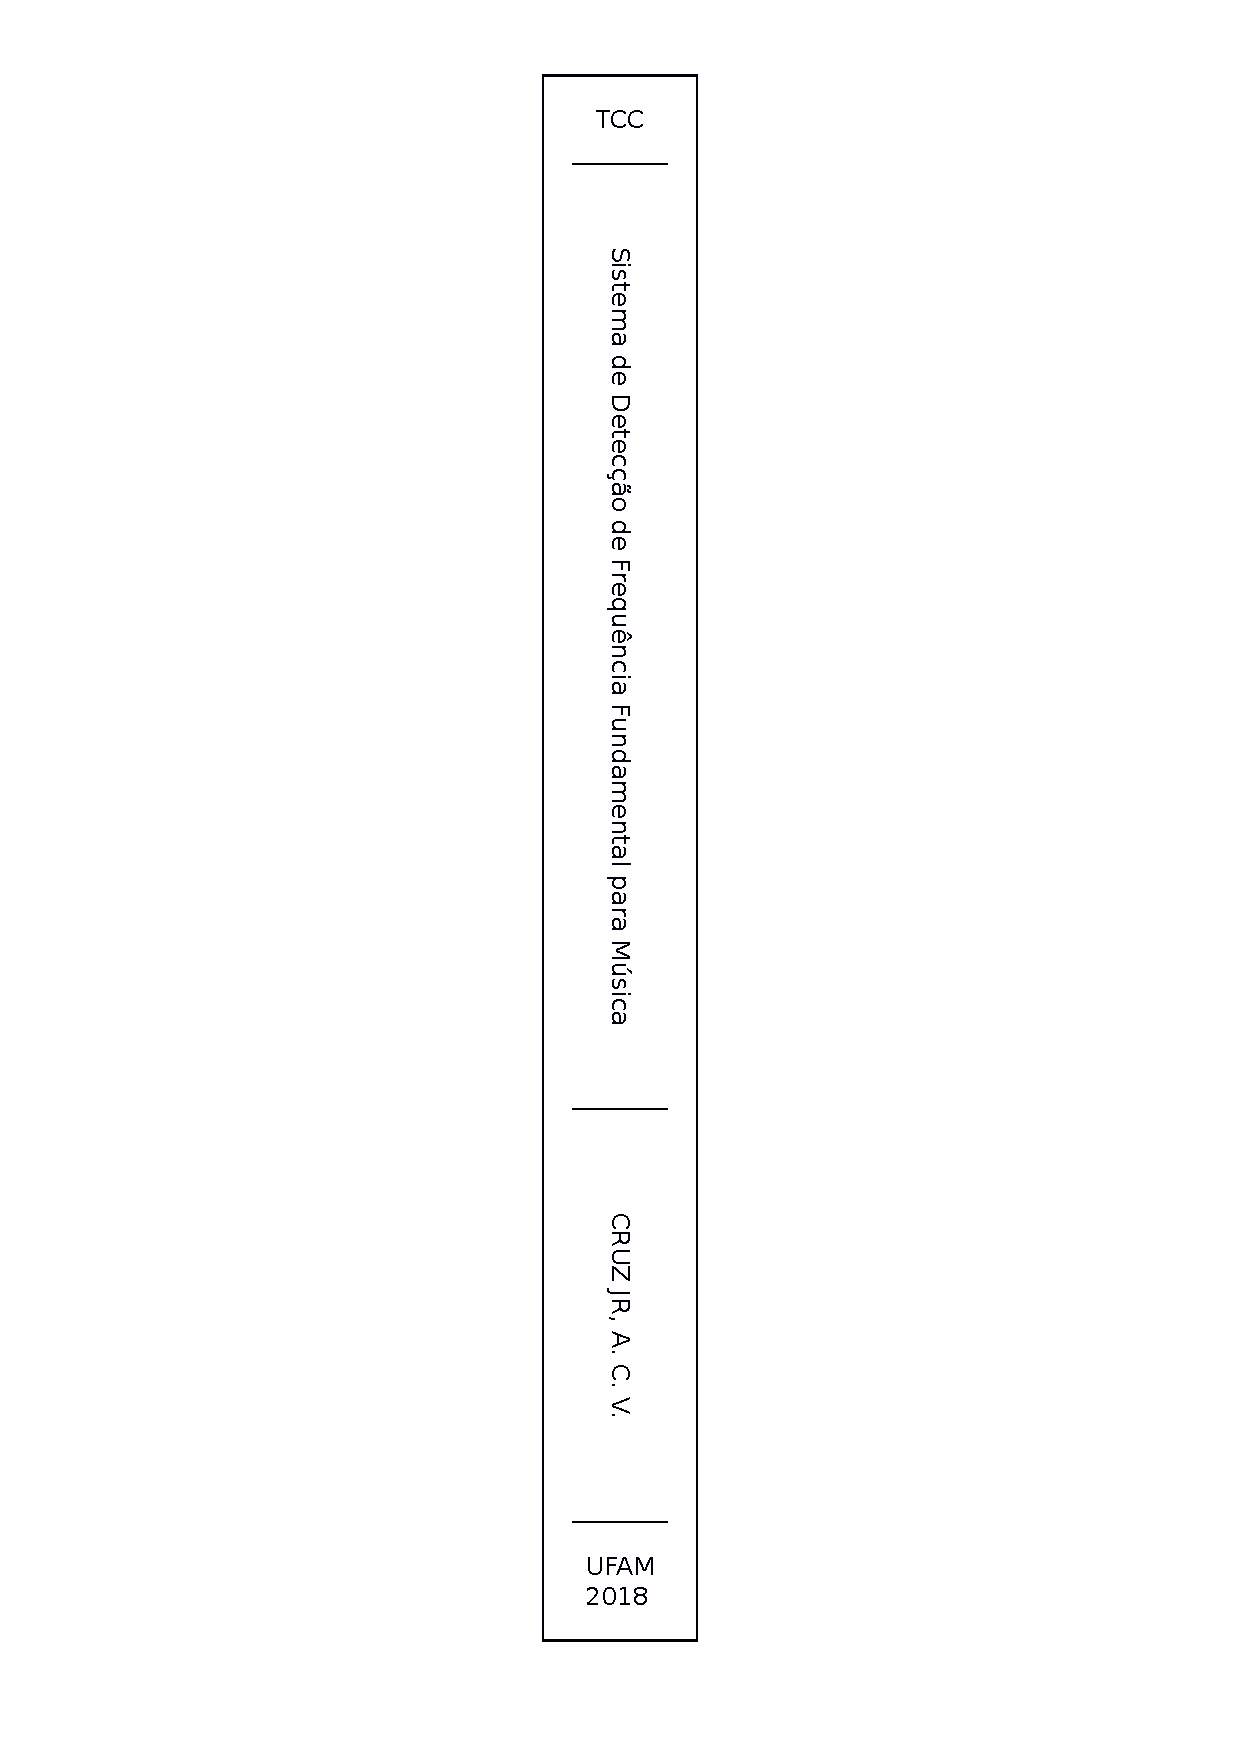
\includepdf{parte1_pre-textuais/lombada_tcc.pdf}
		
\end{titlepage}



\thispagestyle{empty}

\begin{center}

\autor

\vfill {\Large \titulo}

\vfill{
\begin{flushright}
	\begin{minipage}{8cm} 
		\apresentacao
	\end{minipage}
\end{flushright}
}

\vfill Orientador: \orientador

\vfill	\local

\end{center}

\thispagestyle{empty}

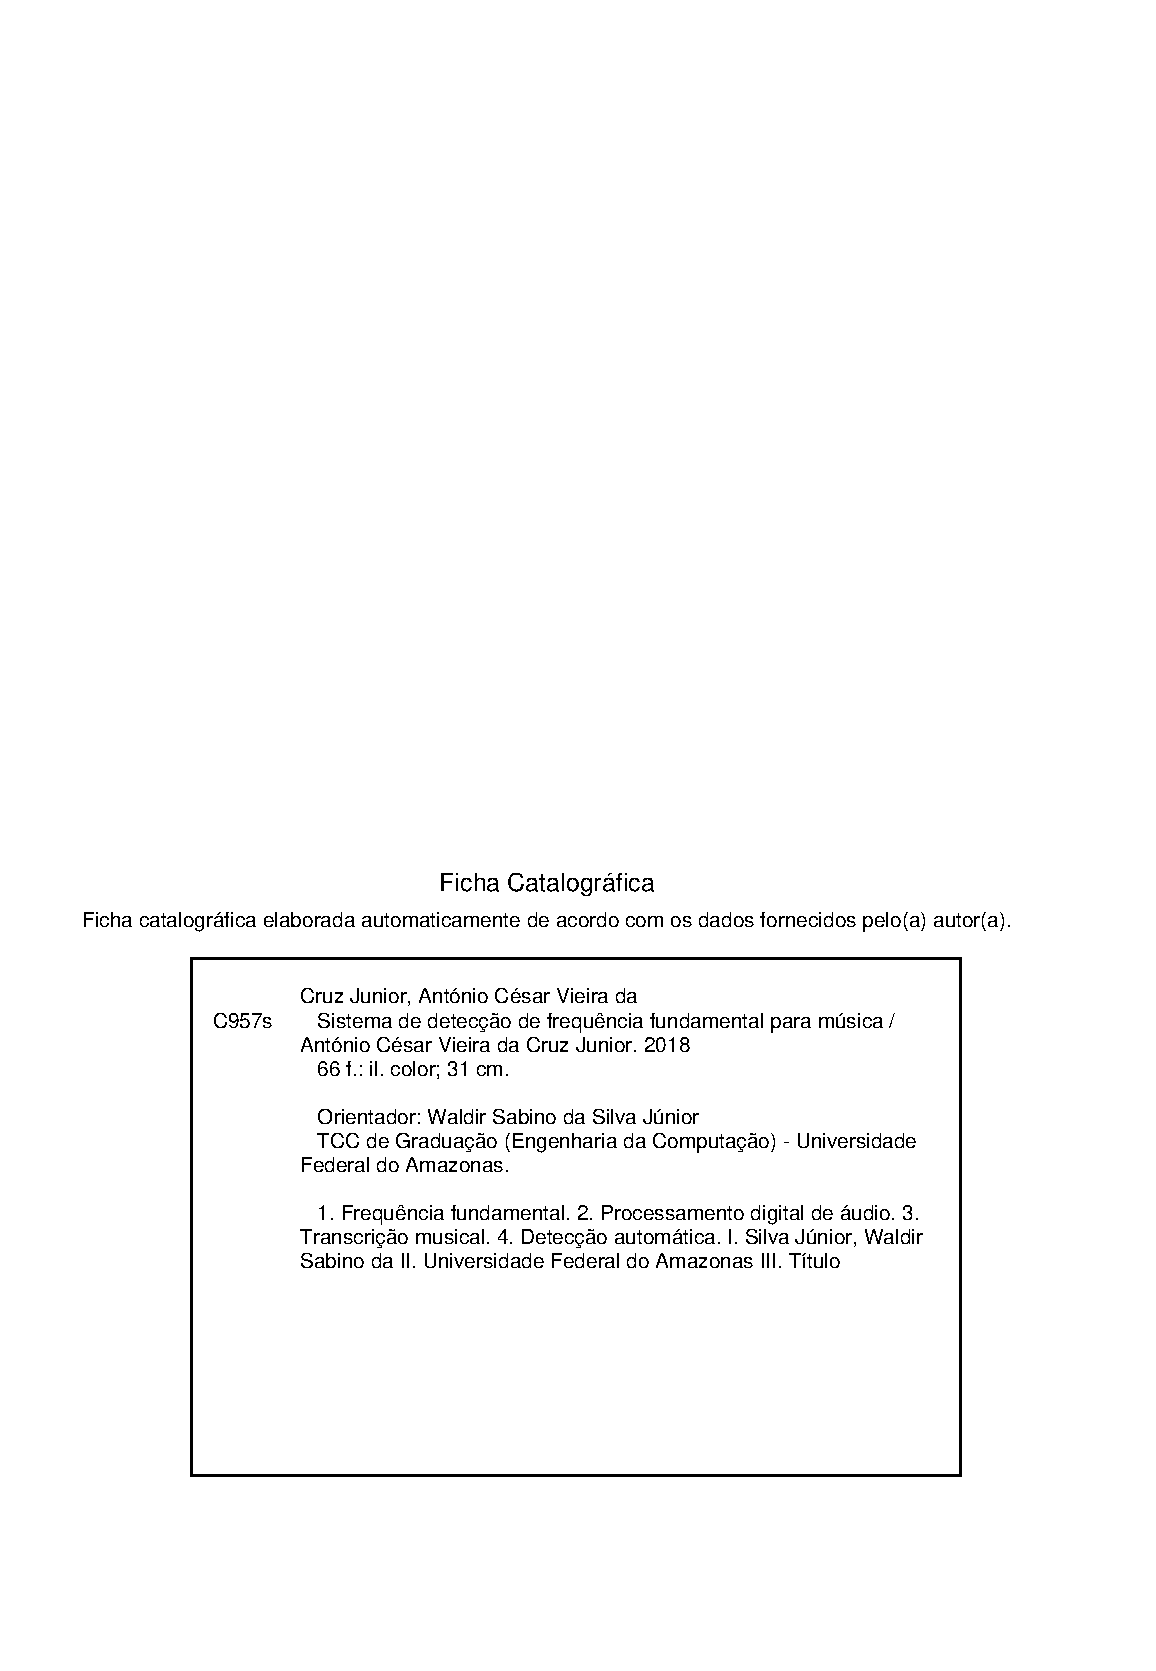
\includepdf{parte1_pre-textuais/ficha_catalografica.pdf}

\thispagestyle{empty}

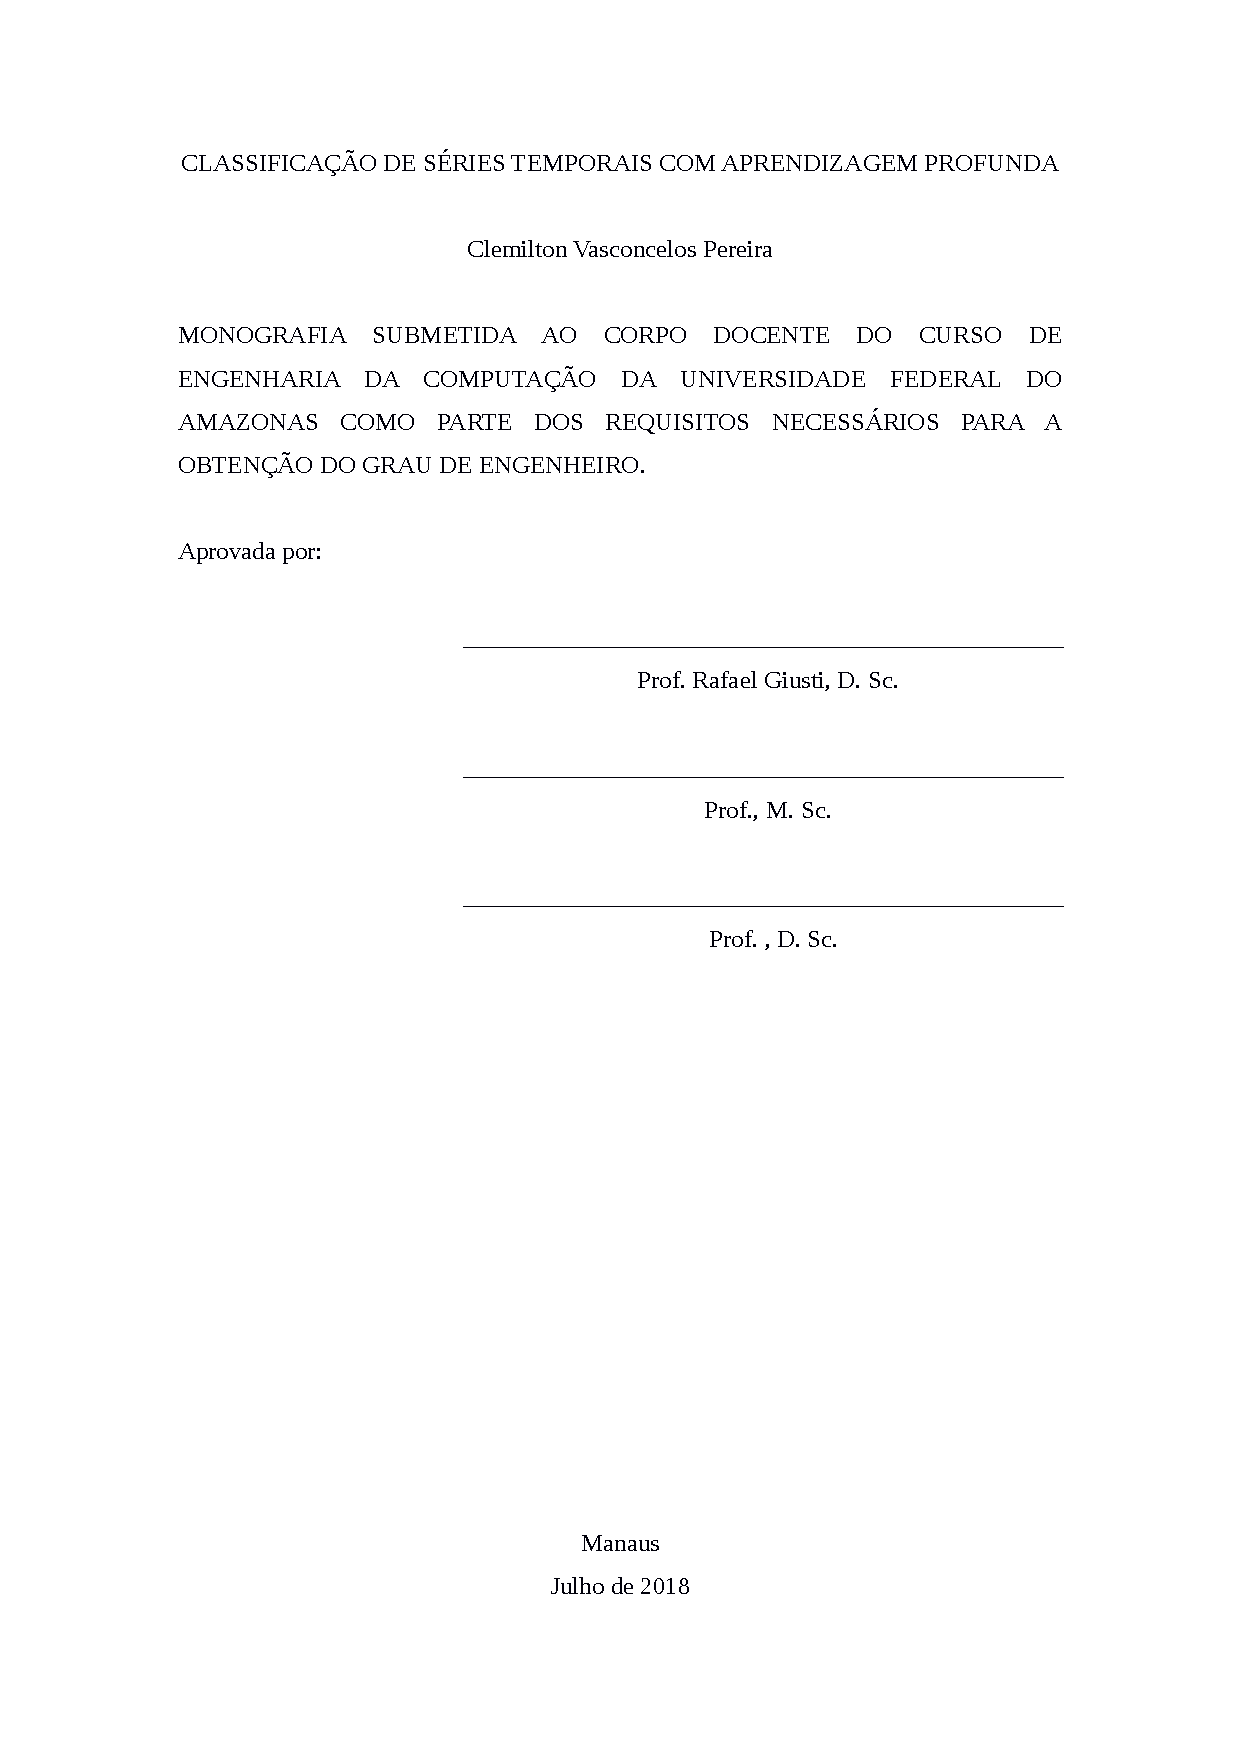
\includepdf{parte1_pre-textuais/tcc_folha_aprovacao.pdf}

\thispagestyle{empty}

\vspace*{\fill}
\begin{flushright}
	\begin{minipage}{8cm}
		\textit{
			\qquad Dedico este trabalho à minha mãe Lúcia, "In memoriam", também aos meus pais, Antonio e Elenir, e às minhas avós Jacyra e Maria, meus exemplos de vida.
		}
	\end{minipage}
\end{flushright}

\chapter*{Agradecimentos}
\thispagestyle{empty}


Antes de tudo, a Deus, autor da vida, cujo a bondade e a misericórdia me seguem a cada dia. Tu és fiel, Senhor!
	

Aos meus pais, Antonio e Elenir, que sempre me apoiaram de todas as maneiras possíveis, à minha amada esposa Yasmin, sempre ao meu lado, e aos meus famíliares, que sempre me incentivaram a persistir.
	

Ao meu orientador, prof. Dr. Waldir Sabino, pela paciência, disposição e direcionamento durante a execução deste projeto, e também pelos conselhos que levo para minha vida profissional.
	

A todos os professores da UFAM, em especial o prof. Dr. César Melo, aos amigos de turma Rosmael, Helton, João Victor, Gabriel, Jordan, Kabashima, Eduardo, Luiz Henrique, Micael e Clemilton, e aos demais amigos e colegas da UFAM pelo convívio, aprendizado e cooperação durante todos esses anos. Vocês foram essenciais nessa caminhada.
	

À família Machado, por todo o cuidado no momento em que mais precisei, e aos irmãos da Segunda Igreja Batista de Manaus, que me adotaram assim que cheguei nesta cidade. Também à Keyseane, que me ajudou em momentos importantes na escrita deste trabalho, e aos meus amigos José Eduardo, Vanessa e Débora.

	
A todos que, de algum modo, colaboraram para que este momento se concretizasse:

\begin{flushright}
	Muito obrigado!
\end{flushright}
\thispagestyle{empty}

\vspace*{\fill}
\begin{flushright}
	\begin{minipage}{8cm}
		\epigraph{``Se algum de vocês tem falta de sabedoria, peça-a a Deus, que a todos dá livremente, de boa vontade; e lhe será concedida.''}{\textit{(Tiago 1.5)}}
	\end{minipage}
\end{flushright}



\chapter*{Resumo}
\thispagestyle{empty}

Existem diferentes caminhos para o reconhecimento automático de uma notas musical, e um deles é por meio da frequência fundamental ($f_0$). Muitas soluções e métodos de detecção automática de $f_0$ já foram desenvolvidas e apresentadas, obtendo resultados positivos. Todavia, é difícil que uma única solução de detecção seja de fato eficaz em ambientes muito diferentes daqueles para o qual a solução foi proposta. Diante disso, o presente projeto aborda o desenvolvimento de um sistema de detecção de $f_0$ para áudios musicais monofônicos, através de processamento digital de sinais, com o intuito de mapear os áudios, fornecendo as frequências fundamentais soadas em cada instante de tempo. Este trabalho também avaliou o sistema desenvolvido, por meio de experimentação a partir de uma base de dados construída para este fim. Percebeu-se que o sistema proposto apresenta boas respostas, sendo necessário melhorias em relação ao tratamento do efeito de ressonância.

\vspace{50pt}

\paragraph{Palavras-chave:} Detecção automática de frequência fundamental, Processamento digital de áudio, Transcrição musical.

\chapter*{Abstract}
\thispagestyle{empty}

There are different ways for a automatic recognition of musical note, one of them is through fundamental frequency ($f_0$). Many solutions and methods of automatic detection of $f_0$ already developed and presented, getting positive results. However, it's hard that one only solution has been effective in environments much different from these that it was proposed. Therefore, the present project approaches the development of a $f_0$ detector system for monophonic musical audios through digital signal processing, with the intention of mapping it, recording the fundamental frequencies sounded at every instant time. This work also evaluated the system developed, through experiments using a database built for it. It was perceived that the proposed system presents good answers, being necessary improvements in the treatment of the resonance effect.
\vspace{50pt}

\paragraph{Keywords:} Automatic Detection of fundamental frequency, Digital Audio Processing, Musical transcription.



\pagenumbering{roman}

\listoffigures

%\thispagestyle{empty}

\listoftables

%\thispagestyle{empty}

\markboth{\MakeUppercase{Lista de Abreviaturas e Siglas}}{\MakeUppercase{Lista de Abreviaturas e Siglas}}

\chapter*{Lista de Abreviaturas e Siglas}

\begin{longtable}{lL{14cm}L{\textwidth}}

\textbf{PDS}  & Processamento Digital de Sinais & \\
\textbf{MIDI}  & Interface Digital de Instrumentos Musicais -- do inglês \textit{\textbf{M}usical \textbf{I}nstrument \textbf{D}igital \textbf{I}nterface} & \\
\textbf{DTFT}  & Transformada de Fourier em Tempo Discreto -- do inglês \textit{\textbf{D}iscret-\textbf{T}ime \textbf{F}ourier \textbf{T}ransform} & \\
\textbf{DFT}  & Transformada Discreta de Fourier -- do inglês \textit{\textbf{D}iscret \textbf{F}ourier \textbf{T}ransform} & \\
\textbf{FFT}  & Transformada Rápida de Fourier -- do inglês \textit{\textbf{F}ast \textbf{F}ourier \textbf{T}ransform} & \\
\textbf{STFT}  & Transformada de Fourier de Tempo Curto -- do inglês \textit{\textbf{S}hort-\textbf{T}ime \textbf{F}ourier \textbf{T}ransform} & \\

\end{longtable}

\markboth{\MakeUppercase{Lista de Símbolos}}{\MakeUppercase{Lista de Símbolos}}

\chapter*{Lista de Símbolos}

\begin{spacing}{1.45}

\noindent \textbf{Símbolos Matemáticos}

\begin{longtable}{L{1.5cm}L{14cm}L{\textwidth}}

$f_s$ & Frequência de amostragem & \\
$f_0$ & Frequência fundamental & \\
$Hz$ & Hertz - Unidade do Sistema Internacional (SI) para frequência & \\
bpm & Batidas por minutos & \\




\end{longtable}

\end{spacing}

\tableofcontents

%\thispagestyle{empty}


\pagenumbering{arabic}

\chapter{Introdução} %Contextualização, motivação e justificativa.

Séries temporais estão presentes em diversos fenômenos ao nosso redor. Tanto em atividades humanas, como em processos naturais, elas têm sido alvo de pesquisas em áreas como clima, economia, medicina, transporte. Além disso, em diversos domínios de pesquisa, dados tipicamente não temporais, como figuras geométricas, a face, mão ou postura corporal de um indivíduo, são representados e analisados como séries temporais. Com o aumento do volume de dados gerados e o avanço nas tecnologias de sensores, houve crescimento no tamanho e na complexidade dos fluxos de dados de séries temporais. Assim, a importância e o impacto das técnicas de análise e modelagem de séries temporais continuam a crescer. 

No contexto da mineração de dados, uma das tarefas mais importantes é a classificação, cujo objetivo é associar cada instância de um conjunto de dados a uma ou mais classes pré-definidas no problema. Para classificação de séries temporais uma característica que não pode ser ignorada é a correlação entre as amostras vizinhas. Com o aumento de dados temporais, centenas de métodos para \textit{TSC} foram propostos desde 2015 \cite{Bagnall2017}. A abordagem mais popular e tradicional é o k-vizinhos mais próximos(KNN) combinada com a distância \textit{Dynamic Time Warping} (DTW). A ideia principal consiste em fazer o cálculo da distância 

O objetivo deste trabalho é avaliar diferentes arquiteturas de aprendizagem profunda para classificação de séries temporais com base no repositório da UCR.

Dentro dessa realidade, o presente projeto aborda o desenvolvimento de um sistema de detecção de f0 para áudios musicais monofônicos, através de processamento digital de sinais, com o intuito de mapear os áudios, fornecendo as frequências fundamentais soadas em cada instante de tempo e identificando os fenômenos aos quais um sistema nesse contexto é submetido. A detecção de f0 será realizada por meio da Transformada de Fourier de Curto Tempo(STFT), considerando f0 como a frequência de maior amplitude dentro de cada janela. Foi construída uma base de dados com áudios de 4 tipos de instrumentos musicais para realização de experimentos, visando validar as detecções realizadas pelo sistema. Este trabalho propõe-se ainda a avaliar a metodologia adotada por meio desses experimentos realizados. 
\section{Organização do Trabalho}



%O texto de introdução deve conter três tipos de informações: apresentação do problema, estado da arte e justificativa do projeto.
%A apresentação ou formulação do problema deve deixar, de forma bem clara, qual será o objeto de estudo do projeto. As razões para a escolha do tema deverão ser justificadas. Desta forma devem ser indicadas: a importância do estudo, quais as possíveis repercussões, quais hipóteses a serem verificadas, entre outras. 
%O estado da arte serve para embasar tanto a formulação do problema como sua justificativa. É preciso situar historicamente a evolução do tema, quais as abordagens já investigadas, qual o estágio atual do conhecimento sobre o assunto ou quais as tendências que se apresentam. Indique as palavras-chave que foram utilizadas para a pesquisa bibliográfica.
%A justificativa do projeto deve indicar por que o projeto deve ser feito, ou seja, por que o problema tratado é relevante. Descreva os fatores de motivação que o(s) levaram a abordar e trabalhar no assunto.
%O final da introdução deve incluir uma descrição de como o documento está estruturado (um parágrafo para indicar o conteúdo de cada seção do Plano do Projeto).

\section{Objetivo}

% Fim Capítulo
\chapter{Fundamentação Teórica} \label{cap2}


Este capítulo aborda, de forma sucinta, os fundamentos teóricos que foram aplicados no planejamento e implementaçao deste projeto.



\section{Aprendizado de Máquina}

Aprendizado de máquina é uma área da inteligência artificial cujo objetivo é o desenvolvimento de técnicas computacionais sobre o aprendizado, bem como a construção de sistemas capazes de adquirir conhecimento de forma automática. Um sistema baseado em aprendizado trabalha por meio de experiências acumuladas e de soluções bem-sucedidas de problemas anteriores  \cite{monard2003}. Normalmente, algoritmos de aprendizado utilizam experiências anteriores, denominadas amostras de treino, para auxiliar no processo de tomada de decisão.  

De acordo com a característica desses casos ou exemplos têm-se três diferentes modos de aprendizado: supervisionado, não-supervisionado e semi-supervisionado. O que distingue esses modos de aprendizado é a presença ou não do atributo classe, que rotula os exemplos do conjunto de dados fornecido ao algoritmo, denominado conjunto de treinamento. No aprendizado supervisionado, esse rótulo é conhecido, enquanto que no aprendizado não-supervisionado os exemplos não estão previamente rotulados. Já no aprendizado semi-supervisionado, o conjunto de treinamento consiste de uns poucos exemplos rotulados e muitos não rotulados\cite{chappelle2006}. O escopo deste trabalho se encontra no aprendizado supervisionado. 


\subsection{Aprendizado Supervisionado}
O objetivo do aprendizado supervisionado é construir um modelo que consegue fazer predição através de instancias de uma base de dados rotuladas. Cada instância da base de dados é representado por um conjunto de características. Na Tabela \ref{table-dataset} é mostrada a estrutura de uma base de dados.
A base de dados é representada por um conjunto $E={E_1,E_2,...,E_N}$  cada instância está relacionada com um rótulo $y_N$. As colunas $A_1$ até $A_N$ se referem as características de cada instância.

A idéia da aprendizagem supervisionada é o conseguir encontrar uma função desconhecida $f$(função conceito) tal que $y=f(\mathbf{x})$, onde o vetor $\mathbf{x}$ são os atributos de uma instância específica. Na prática, a função $f$ deve conseguir prever o valor correto $y_i$ de uma instância $E_i$ não vista. Quase sempre, o número de exemplos da base de dados não é suficiente para descrever a função conceito. Nesse caso, o classificador é visto como uma hipótese $h$ que aproxima $f$, ou seja, $h(x)\approx f(x)$ . Caso os valores dos rótulos $y_1,y_2,...,y_N$ sejam numéricos o problema é denominado de \textit{regressão}, caso sejam valores categóricos o problema é denominado de \textit{classificação}. 

\begin{table}[]
	\centering
	\begin{tabular}{c|cccc|c}
		\hline
		& $A_1$ & $A_2$ & \dots & $A_M$  & Classe(Y) \\
		\hline 
		\hline
		$E_1$ & $x_{11}$ & $x_{12}$ & \vdots & $x_{1M}$ & $y_1$ \\
		$E_2$ & $x_{21}$ & $x_{22}$ & \vdots & $x_{2M}$ & $y_2$ \\
		\vdots & \vdots & \vdots &  $\ddots$ & \vdots & \vdots \\
		$E_N$ & $x_{N1}$ & $x_{N2}$ & \vdots & $x_{NM}$ & $y_N$ \\
		\hline
		
		
	\end{tabular}	
	\caption{Representação da base de dados}
	\label{table-dataset}
\end{table}


De maneira geral, a base de dados é dividida em dois conjuntos: conjunto de \textit{treino} e conjunto de \textit{teste}. O conjunto de treinamento é utilizado para ajustar o classificador. Como dito anteriormente, o classificador é uma hipótese da função conceito $f$ ,logo, é fundamental que o conjunto de treinamento tenha uma distribuição o mais semelhante possível do conjunto original.  O conjunto de teste é utilizado para avaliar o modelo construído. Idealmente, esse conjunto não deve ter exemplos em comum com o conjunto de treinamento.

Em alguns casos, pode ser necessário utilizar um conjunto de \textit{validacao}, extraído do conjunto de treinamento, para realizar ajustes no modelo construído pelo algoritmo de aprendizado. Logo tem-se três conjuntos: \textit{treino}, \textit{validação} e \textit{teste}. O treino é utilizado para aprendizagem do algoritmo. O modelo é avaliado através do conjunto de validação. É feita uma alteração dos parâmetros do classificador e outro treinamento é realizado. O intuito é melhorar o desempenho do modelo, através desses "ajustes". Dessa maneira os exemplos de validação são indiretamente "vistos" durante o processo de aprendizado, o que obriga que esses exemplos sejam diferentes dos exemplos de testes.

\subsection{Normalização e One-Hot Enconding}
Os algoritmos de aprendizagem de máquina aprendem através dos dados. Dados do mundo real apresentam valores que estão em distintas faixas. A fim de evitar que algum atributo predomine sobre outro ou que incluar alguma ponderação indesejada ao induzir um modelo e AM, é comum fazer uma normalização dos valores de cada atributo. Um forma de normalizar os dados é mostrada na Equação \ref{eq-norm}:

\begin{equation}\label{eq-norm}
x_{ij} = \frac{x_{ij} - \overline{x}}{ \sigma_j}
\end{equation}

onde $\overline{x}$ representa a média do atributo e $\sigma_j$ representa o desvio padrão.

Os algoritmos de AM geralmente possuem como entrada e saída valores numéricos, portanto é necessário converter os valores categóricos do dataset para valores numéricos. A codificação one-hot é um processo que converte rótulos em vetores binários como mostrado na Figura \ref{fig-onehot}. Uma vantagem dessa codificação é que não cria uma "ordem" numérica nos dados. Essa ordem poderia interferir na indução do classificador, podendo dar maior importância para valores maiores, o que não faz sentido para variáveis categóricas.

\begin{figure}[h]
	\centering
	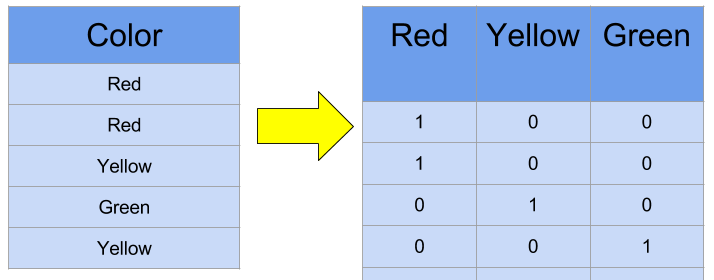
\includegraphics[scale=0.5]{pasta1_figuras/one-hot.png}
	\caption{Codificação One-hot}
	\label{fig-onehot}
\end{figure}

\subsection{K-Nearest Neighbors (KNN)}
Um classificador bastante popular é o K-Nearest Neighbors(K-Vizinhos mais próximos). O k-NN utiliza os próprios dados de treinamento como modelo de classificação, isto é, para cada novo exemplo teste que se deseja classificar, utiliza-se os dados de treinamento para verificar  quais são as instâncias de treino "mais próximas" do exemplo de teste. O exemplo teste é classificado com a mesma classe dos seus vizinhos mais próximos. A cada nova exemplo a ser classificado faz-se uma varredura nos dados de treinamento, o que provoca um grande esforço computacional

O princípio do classificador k-NN é a ``regra dos vizinhos mais próximos''. A hipótese é que, dado um conjunto de exemplos distribuídos sobre o espaço de dados $X$, a ``vizinhança'' de um exemplo $x \in X$ estabelecida por uma função de distância apropriada tende a ser ocupada por exemplos que pertencem à mesma classes que $x$ \cite{hart1967} , como ilustrado na Figura \ref{fig-knn}. Desse modo a informação fornecida pelos exemplos conhecidos que são mais similares a $x$.

\begin{figure}[h]
	\centering
	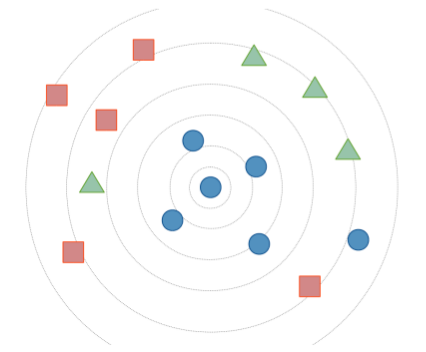
\includegraphics[scale=0.5]{pasta1_figuras/knn.png}
	\caption{Princípio dos k-vizinhos mais próximos}
	\label{fig-knn}
\end{figure}

Para encontrar os vizinhos mais próximos é necessário definir uma medida de similaridade entre dois exemplos. Uma medida de similaridade bastante popular é a \textit{distância euclidiana}. Tal medida calcula a raiz quadrada da norma do vetor diferença entre os vetores $x$ e $y$:
\begin{equation} \label{eq_disteucli}
d(x,y)= \sum_{i=1}^{K} (x_i - y_i)^2
\end{equation}

\section{Redes Neurais Artificiais}
Redes Neurais Artificais são modelos computacionais que buscam simular o processamento de informação pelo cérebro humano. Elas são compostas por unidades simples de processamento, os neurônios, que se unem por meio de conexões sinápticas \cite{zhang1998}. Cada conexão, além de ser altamente especializada, é responsável pelo envio de sinais de um neurônio para outro. Segundo \cite{haykin2009}, os neurônios e suas conexões podem ser implementados utilizando-se de componentes eletrônicos ou via simulação programada em computador.

\subsection{Inspiração Biológica e Perceptron}

Um bloco básico de uma rede neural tem algumas semelhanças com um neurônio biológico. O neurônio biológico é uma célula formada por três seçoes com funções específicas e complementares: \textit{corpo},\textit{dentritos} e \textit{axônio}. Os dentritos captam os estímulos recebidos em um determinado período de tempo e os transmitem ao corpo do neurônio, onde são processados. Quando tais estímulos atingirem determinado limite, o corpo da célula envia um novo impulso que se propaga pelo axônio e é transmitido às células vizinhas por meio de sinapses.  Este processo pode se repetir em várias camadas de neurônios. Como resultado, a informação de entrada é processada, podendo levar o cérebro a comandar reações físicas.  \cite{ferneda2006}. A figura \ref{fig-neuronio} ilustra de forma simplificada as partes de um neurônio.

\begin{figure}[h]
	\centering
	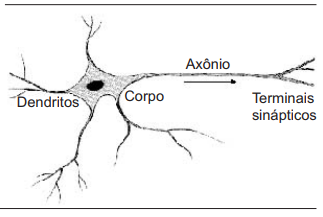
\includegraphics[scale=0.5]{pasta1_figuras/neuronio.png}
	\caption{Representação simplificada de um neurônio}
	\label{fig-neuronio}
\end{figure}

O modelo de um neurônio artifical é apresentado na Figura \ref{fig-guide-1}. Este modelo é composto por três elementos:
\begin{itemize}
	\item Um cojunto de entradas $(x_1,x_2,...,x_n)$ que são multiplicadas por um conjunto e pesos $(p_1,p_2,...,p_n)$;
	\item Um somador $(\sum)$ para acumular o sinais de entrada;
	\item Uma função de ativação que ($\varphi$) limita o intervalo permissível de amplitude do sinal de saída (y) a um valor fixo.
\end{itemize}

\textbf{\begin{figure}[h]
	\centering
	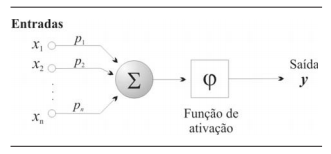
\includegraphics[scale=0.6]{pasta1_figuras/perceptron.png}
	\caption{Modelo matemátiico de um neurônio}
	\label{fig-perceptron}
\end{figure}}

Esse modelo foi proposto por \textit{McCulloch and Pitts} em 1943 \cite{McCulloch1943} e é conhecido como \textit{perceptron}. A função de ativação ($\varphi$) tem a seguinte definição:
\begin{equation} \label{eq_activation}
\varphi = \left\{ \,
\begin{IEEEeqnarraybox}[][c]{l?s}
\IEEEstrut
1 & if $\sum_{i=1}^{n} p_i x^k_i \geq T$, \\
0 & if $\sum_{i=1}^{n} p_i x^k_i < T$ 
\IEEEstrut
\end{IEEEeqnarraybox}
\right.
\end{equation}
Os valores dos pesos podem ser positivos ou negativos e eles refletem se aquela conexão é inibitória ou excitatória. Um valor positivo ou negativo reflete a importância da respectiva entrada para o processamento. Frequentemente é adicionado um \textit{viés} $b$ na entrada da função de ativação. A forma geral do modelo é descrito como:
\begin{equation} \label{eq-output-percep}
y(k) = \varphi(\sum_{i=1}^{n} p_i(k) x_i(k) +b(k))
\end{equation}
Os pesos sinápticos do Perceptron podem ser adaptados empregando um processo de aprendizado com um número finito de iterações. A aprendizagem é conduzida pela regra de correção de erro conhecida como algoritmo de convergência do Perceptron. Esse algoritmo visa encontrar um vetor de pesos w tal que as duas igualdades da função degrau sejam satisfeitas(\textit{Lippmann}, 1987 \cite{lippman1987})

\subsection{Perceptron multicamadas}

O Perceptron multicamadas(\textit{Multi-Layer Perceptron - MLP}) é uma generalização da rede perceptron. Novas camadas são adicionadas o que possibilita a solução de problemas que não sejam linearmente separáveis. O vetor de entradas \textbf{x} passa pela camada inicial, cujos valores de saída são ligados a camada seguinte. Esse processo se repete até chegar na última camada.(Figura \ref{fig-mlp})  Pode-se arranjar a rede em várias camadas, tornando-a profunda e capaz de aprender relações cada vez mais complexas.

\begin{figure}[h]
	\centering
	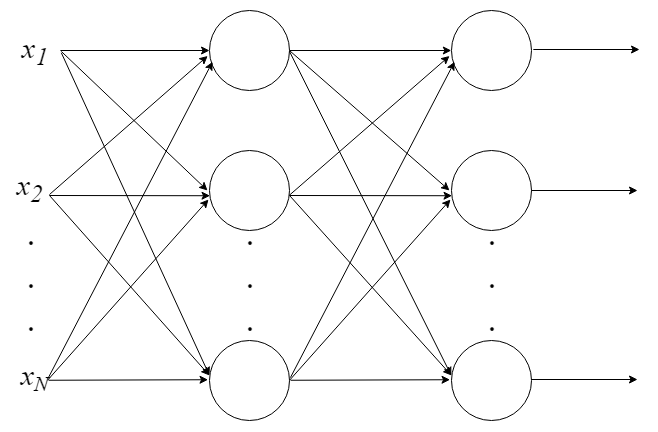
\includegraphics[scale=0.4]{pasta1_figuras/mlp.png}
	\caption{Multilayer Perceptron. Cada círculo representa um neurônio mostrado anteriormente}
	\label{fig-mlp}
\end{figure}

Em 1986, \textit{Rumelhart, Hinton e Williams} \cite{hinton1986} desenvolveram o algoritmo \textit{backpropagation}, que utiliza o gradiente descendente para treinar uma MLP. Este método é composto pelas fases \textit{forward} e \textit{backward}.O objetivo do backpropagation é otimizar os pesos para que a rede neural possa aprender a mapear corretamente as entradas para as saídas. A primeira fase é a ``propragação adiante'' (forward), onde as entradas inseridas na rede se propagam entre as camadas, uma a uma, até a produção das respectivas saídas, portanto a função dessa fase é gerar uma resposta considerando as entradas e os respectivos pesos sinápticos, os quais permanecem inalterados.

Na fase backward é onde a aprendizagem dos pesos é realizada. Esse aprendizado se dá através da otimização (minimização) da função loss, a qual determina a qualidade da classificação do dado de entrada.Essa otimização é realizada através de um método chamado \textit{Gradiente Descendente} que busca a minimização da função \textit{loss} ao alterar os pesos na direção de maior declive do gradiente. O gradiente é calculado na última camada e então é retro-propragado para as camadas intermediárias anteriores que contribuem diretamente para a formação da saída. Cada elemento da camada intermediária recebe é responsável apenas por uma porção do gradiente total.Este processo se repete, camada por camada, até que cada elemento tenha a sua parcela de gradiente para o gradiente total. Baseado no gradiente, é feita uma alteração dos valores dos pesos e bias de modo que a rede aprenda os padrões do conjunto de treinamento.



\subsection{Camada Softmax}

Como explicado em \textit{GoodFellow, Bengio, e Courville}(2016 \cite{Goodfellow2016}), a camada softmax é utilizada como um classificador na camada de saída e tem como objetvio representar a probabilidade de cada classe para cada valor de entrada.

Pela Equação 3.5 nota-se que os valores de saída da camada softmax estão entre 0 e 1, e que a soma de de todas as saídas é igual a 1. Desta forma, cada neurônio de saída representa representa a probabilidade da entrada pertencer a uma determinada classe.

\begin{equation}
softmax(z_i) = \frac{exp(z_i)}{\sum_{j}^{} exp(z_j)}
\end{equation}


\subsection{Hiperparâmetros de uma Rede Neural}
A maioria dos algoritmos de AM envolvem "hiperparâmetros", que são varíaveis definidas para o algoritmo antes do treinamento com o objetivo de otimizá-lo. Definir os valores de hiperparâmetros pode ser visto como uma seleção de modelos, ou seja, escolher qual modelo usar do conjunto hipotético de modelos possíveis. Em redes neurais os hiperparâmeteros determinam a estrutura da rede (Ex: Número de neurônios em uma camada) ou como a rede será treinada(Ex: Taxa de aprendizado)

\subsubsection{Mini-batches}
O treinamento geralmente é realizado em \textit{batches} também conhecidos como \textit{mini-batches} que são subconjuntos do treino. As razões de utilizar batches e não o treino inteiro são: diminuição do tempo de treinamento; caso o conjunto de treino seja suficientemente grande, uma amostra desse conjunto pode representar de forma \textit{boa} o conjunto original. A tamanho dessa amostra é um hiperparâmetro da rede, sendo geralmente aceito que o treinamento com \textit{batches} maiores resulta numa melhor performance.

\subsubsection{Taxa de aprendizado}
A taxa de aprendizado  determina o quão ``rápido" as atualizações dos pesos irão em direção do gradiente. Se a taxa de aprendizado for muito pequena, o modelo convergirá muito lentamente; Se a taxa de aprendizado for muito grande, o modelo irá divergir. 




\section{Séries Temporais}

Série temporal é uma sequência de observações de um fenômeno ao longo do tempo. Geralmente essas medições são feitas em um intervalo de tempo regular. A ordem das amostras é crucial, pois há um dependência entre os dados e uma alteração da ordem pode modificar o significado dos dados. Uma série temporal pode ser definida como:

\begin{equation} \label{eq_TS}
X(t) = (x_1,x_2,...,x_n)
\end{equation}
onde $x_n$ representa uma observação no instante $t$, $n$ o número de observações e $X(t)$ a função que descreve a série temporal em termos de t. Caso a série seja constituída de uma observação em cada instante de tempo ela é chamada de \textit{univariada}. Caso a série foi obtida por uma coleta simultânea de dois ou mais fenômenos ela é chamada de \textit{multivariada}.

As séries temporais estão em diversas áreas do conhecimento como Economia (preços diários dea ações, taxa mensal de desemprego, produção industrial), Medicina (eletrocardiograma, eletroencefalograma), Epidemiologia (número mensal de novos casos de meningite), Meteorologia( precipitação pluviométrica, temperatura diária, velocidade do vento).

\subsection{Aplicações de Séries Temporais}
A análise de séries temporais tem atraído muitos pesquisadores em aprendizado de máquina ao redor do mundo. As principais tarefas envolvendo séries temporais na qual se utiliza aprendizagem de máquina são as seguintes:

\begin{itemize}
	\item \textit{Classificação}: cada série temporal representa uma classe distinta de objetos. Dada uma série temporal, o objetivo é descobrir qual é a classe de objetos ela representa; 
	\item Agrupamento: Dado um conjunto de séries temporais, o objetivo é encontrar uma estrutura natural que permita distribuir as séries em grupos; 
	\item Detecção de Motivos: também conhecido como detecção de \textit{motifs}; o objetivo é encontrar uma ou mais subsequências que aparecem frequentemente na séries;
	\item Detecção de Anomalias: encontrar subsequências ou séries que são inesperadas em algum contexto.
\end{itemize}
Este trabalho está inserido na tarefa de classificações de séries temporais.
\section{Classificação de Séries Temporais}


\section{Frequência Fundamental}

A frequência fundamental $f_0$ é a menor frequência de uma vibração, ou também, a primeira frequência de uma série harmônica. Uma série harmônica é o conjunto de ondas composto pela $f_0$ e suas múltiplas inteiras. Normalmente, todo estímulo sonoro é formado por uma série harmônica. A frequência fundamental está diretamente ligada à altura de um som e, por meio dela, distingue-se grave e agudo.


\section{Pitch}


O $pitch$ é um conceito musical relacionado à frequência fundamental, entretanto voltado para a percepção humana do som. Ele é definido em \cite{hartmann1996} como \textit{``o atributo pelo qual a audição pode ordenar os sons em uma escala de grave para agudo, dependendo principalmente do conteúdo de frequência do estímulo sonoro, mas também da forma de onda desse estímulo''}. Embora pareça confusa, esta definição abrange a relação do $pitch$ com a altura e com o timbre de um som, necessário para que o conceito seja válido em todos os casos, tanto em aplicações musicais como em aplicações de reconhecimento de fala. Em \cite{klapuri2006}, fica evidente que o $pitch$ de um som refere-se a frequência em que uma onda senoidal é reconhecida por um ouvido humano como correspondente ao som em questão.


\section{Detecção Automática de $f_0$}

Embora muitos trabalhos tratem frequência fundamental e $pitch$ como sinônimos, \cite{gerhard2003} explica de modo claro que existem diferenças consideráveis entre os dois conceitos, de modo que um sistema de detecção de $pitch$ objetiva resultados diferentes de um sistema de detecção de $f_0$. Como exemplo disso, pode-se observar que um sinal com frequências mais puras e poucas informações de timbre são ideais para a detecção de $f_0$, entretanto, a detecção de $pitch$ depende ainda da intensidade, duração e timbre.


Muitas soluções e métodos de detecção automática de $f_0$ já foram desenvolvidas e apresentadas, obtendo resultados positivos. Entretanto, \cite{gerhard2003} também afirma que é difícil que uma mesma solução de detecção de $f_0$ tenha bom desempenho tanto aplicações de música quanto em aplicações de fala. Deste modo, primeiro torna-se necessário definir o tipo de aplicação do sistema de detecção para, só então, desenvolver e avaliar o desempenho desse sistema no contexto escolhido.


\section{Digitalização de um Sinal de Som}

Para a digitalização de um sinal sonoro, são necessários a amostragem, a quantização e a codificação. 

\subsection{Amostragem}
A amostragem é o processo de conversão de um sinal contínuo no tempo em um sinal discreto. Se a discretização no tempo ocorrer em uma frequência de amostragem ($f_s$) muito baixa, as altas frequências não serão amostradas, gerando o efeito \textit{aliasing}, que é a distorção de um sinal causado pela perda das informações de alta frequência. 


Segundo o Teorema da Amostragem\cite{lathi2007}, dado um sinal contínuo amostrado com frequência $f_s$, se $f_s > 2f_M$, onde $f_M$ é a frequência máxima do sinal, então será possível recuperar toda a informação do sinal a partir dos valores amostrados. O intervalo entre a coleta de cada amostra é denominado \textit{período de amostragem}, representado pelo símbolo $T_s$. Pela relação de período e frequência, temos que $T_s = \frac{1}{f_s}$.


A Figura \ref{fig-sampling} demonstra graficamente a amostragem de um sinal.


\subsection{Quantização}
A quantização, por sua vez, consiste em selecionar um conjunto de valores finitos, espaçados linearmente ou não, para os quais as amostras terão seus valores de amplitude arredondados. A diferença entre o valor real e o valor quantizado da amostra é chamado de erro de quantização. Na digitalização de sinais, deve-se adotar um conjunto de quantização com tamanho suficientemente grande para que as perdas de informação por erros nesse procedimento não impeçam uma posterior recuperação do sinal.


A Figura \ref{fig-quantizacao} demonstra graficamente a quantização de um sinal.

\begin{figure}[h]
	\begin{subfigure}{0.5\textwidth}
		\centering
		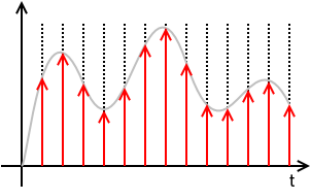
\includegraphics[scale=0.4]{pasta1_figuras/amostragem.png}
		\caption{Amostragem} \label{fig-sampling}
	\end{subfigure}
	\hspace*{\fill} % separation between the subfigures
	\begin{subfigure}{0.5\textwidth}
		\centering
		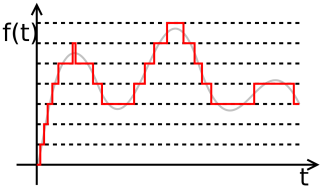
\includegraphics[scale=0.75]{pasta1_figuras/quantization.png}
		\caption{Quantização} \label{fig-quantizacao}
	\end{subfigure}
	\caption{Amostragem e Quantização}
\end{figure}

\subsection{Codificação}
Por fim, a codificação é o procedimento no qual se define o formato de armazenamento das informações do sinal. Após esse passo, essa representação digital passa a ser denominada áudio. Existem diferentes codificadores para áudio, cada um deles com suas particularidades. Alguns codificadores usam técnicas de compressão, que podem gerar pequenas perdas de informação, enquanto outros buscam preservar a integridade da representação, sendo, consequentemente, maiores em tamanho de arquivo. O Matlab\rreg trabalha nativamente com 8 tipos de codificadores de áudio: \textit{WAVE, OGG, FLAC, AU, AIFF, AIFC, MP3 e MPEG-4 AAC}\cite{mathworks2018audioread}.


\section{Notas Musicais}

Sob a ótica da música, os \textit{pitches} são representados pelas notas musicais. A distância entre a frequência de uma nota e metade ou dobro dessa mesma frequência é chamada de oitava. O menor intervalo entre duas notas é chamado de ``semitom'', enquanto um ``tom'' são dois semitons. A Tabela \ref{tab-notas} exibe todas as notas da 4ª oitava. A nota Lá (A) nessa oitava equivale a frequência de 440Hz, isso significa que essa mesma nota na 3ª oitava tem metade dessa frequência, ou seja, 220Hz. Por padrão, a nota lá da 4ª oitava, ou A4, é usada como base para a definição de todas as outras notas. A maioria dos músicos utiliza A4 em 440Hz, mas há casos em que são adotadas frequências diferentes como 436Hz e 444Hz.

\begin{table}[]
	\centering
	\begin{tabular}{|c|c|c|}
		\hline
		\textbf{Nota}                                           & \textbf{Abreviação} & \textbf{Frequência (em Hz)} \\ \hline
		Dó                                                      & C                   & 261.6                       \\ \hline
		\begin{tabular}[c]{@{}c@{}}Dó Sustenido ou Ré Bemol\end{tabular}  & C\# ou Db                 & 277.2                       \\ \hline
		Ré                                                      & D                   & 293.7                       \\ \hline
		\begin{tabular}[c]{@{}c@{}}Ré Sustenido ou Mi Bemol\end{tabular}  & D\# ou Eb                 & 311.1                       \\ \hline
		Mi                                                      & E                   & 329.6                       \\ \hline
		Fá                                                      & F                   & 349.2                       \\ \hline
		\begin{tabular}[c]{@{}c@{}}Fá Sustenido ou Sol Bemol\end{tabular}  & F\# ou Gb                 & 370.0                       \\ \hline
		Sol                                                     & G                   & 392.0                       \\ \hline
		\begin{tabular}[c]{@{}c@{}}Sol Sustenido ou Lá Bemol\end{tabular} & G\# ou Ab                 & 415.3                       \\ \hline
		Lá                                                      & A                   & 440.0                       \\ \hline
		Lá Sustenido ou Si Bemol                                            & A\# ou Bb                 & 466.2                       \\ \hline
		Si                                                      & B                   & 439.9                       \\ \hline
	\end{tabular}
	\caption{Notas musicais da 4ª oitava e suas frequências}
	\label{tab-notas}
\end{table}


\section{Ressonância}


A ressonância é um fenômeno físico em que uma vibração dá origem a outras vibrações com maior amplitude em um conjunto de frequências específicas. Essas frequências geradas são chamadas de frequências ressonantes. Os instrumentos musicais também podem apresentar esse fenômeno, como, por exemplo, alguns instrumentos de corda (violão, piano acústico, violino, entre outros) que utilizam uma caixa de ressonância para amplificar o som gerado pela vibração de suas cordas.


\section{Domínios}

Em PDS, os sinais são representados em dois diferentes domínios: tempo e frequência. No domínio do tempo, ou domínio temporal, um sinal é representado como amostragens de sua amplitude em intervalos de tempo $T$. Já no domínio da frequência, ou domínio espectral, um sinal é representado pela amplitude das oscilações que ocorrem em cada frequência. Desse modo, ter o mesmo sinal em diferentes domínios é tê-lo em diferentes perspectivas.


Os domínios do tempo e da frequência são permutáveis entre si, ou seja, dado um sinal $x(t)$ temporal, é possível transportar esse sinal para a representação espectral na forma $X(j\omega)$ sem que haja perda da informação. Do mesmo modo, é possível fazer o caminho inverso e retornar um sinal na frequência para a sua forma temporal inicial. Para transitar entre os domínios, utiliza-se as transformadas de Fourier.

\section{Transformada de Fourier}

A transformada de Fourier é uma ferramenta de decomposição de uma função em partes de base senoidal, ou seja, o sinal temporal passa a ser expresso em frequências. Inicialmente proposta pelo francês Jean Baptiste Joseph Fourier\cite{open1999}, as séries de Fourier deram origem a diferentes versões da transformada de Fourier, cada uma voltada para um tipo de sinal de origem.



Para sinais discretos no tempo utiliza-se a Transformada de Fourier em Tempo Discreto (DTFT, do inglês \textit{Discrete-Time Fourier Transform}), dada pela equação (\ref{eq_DTFT}):

\begin{equation} \label{eq_DTFT}
	X(\omega) = \sum_{n=-\infty}^{+\infty}x(n)e^{-j\omega n}
\end{equation}
onde $\omega$ é a frequência angular, em radianos por segundos, e $n$ é a posição da enésima amostra do sinal.


A DTFT é aplicável a sinais discretos no tempo, entretanto, é computacionalmente inviável, visto que sua saída é contínua na frequência. Deste modo, torna-se necessário discretizar essa saída para valores específicos de $\omega$. Para este fim, desenvolveu-se a Transformada Discreta de Fourier (DFT, do ingês \textit{Discrete Fourier Transform}).


\section{Transformada Discreta de Fourier}


A DFT é dada pela equação (\ref{eq_DFT}):

\begin{equation} \label{eq_DFT}
	X(k) = \sum_{n=0}^{N-1}x(n)e^{-j2\pi \frac{kn}{N}}
\end{equation}
onde x(n) é um sinal finito de tamanho N, e k assume valores inteiros de 0 a N-1.


Nesse contexto, X(k), DFT do sinal de entrada, é uma saída periódica. Essa discretização da saída aproxima a transformação de Fourier para a viabilidade computacional. Entretanto, executar uma soma do tamanho do sinal sob análise para cada valor específico da DFT,  ainda demanda um grande trabalho computacional, pois à medida em que aumenta-se o sinal de entrada, também aumenta-se quadraticamente a quantidade de operações. Por notação assintótica, pode-se afirmar que a DFT exige um esforço computacional $\Omega(N^2)$.


Por esse motivo, tornou-se necessário obter um algoritmo computacionamente mais eficiente para calcular a DFT: A Transformada Rápida de Fourier (FFT, do inglês \textit{Fast Fourier Transform}).


\section{Transformada Rápida de Fourier}

Designa-se como FFT uma série de algoritmos propostos que visam realizar a DFT de maneira mais eficiente. A Transformada Rápida de Fourier reduz as operações computacionais de $\Omega(N^2)$ para $\Omega( N log_2 N)$, tornando viável tal implementação. Para o presente projeto, utilizou-se a função nativa \textit{fft} do MATLAB\rreg, cujo a documentação fornece também casos básicos de uso\cite{mathworks2018}. Essa implementação baseia-se na equação:

\begin{equation} \label{eq-fft-matlab}
	X(k)=\sum_{j=1}^{N}x(j) W(N,j,k)
\end{equation}
onde $x(n)$ é o sinal de entrada, $N$ o tamanho do sinal, e $W$ é dado como:
\begin{equation} \label{eq-fft-matlab-w}
	W(N,j,k) = cos(\frac{2\pi i(j,k)}{N}) + j sen(\frac{2\pi i(j,k)}{N})
\end{equation}
onde,
\begin{equation} \label{eq-fft-matlab-i}
	i(j,k) = (j-1)(k-1)
\end{equation}

O tempo de execução dessa função depende do tamanho da entrada. Sinais com comprimentos que sejam potências de 2 são mais rápidos para o processamento, seguidos pelos sinais cujo o comprimento contém apenas pequenos fatores primos. As entradas que demoram mais para serem processadas são aquelas em que seu comprimento contém grandes fatores primos.


O tamanho e a precisão na frequência da saída de um algoritmo FFT também está diretamente relacionado ao tamanho do sinal de entrada. Em casos onde o sinal a ser transformado não possui um tamanho ideal para a precisão no domínio da frequência e tempo de execução desejados, pode-se adotar a técnica de \textit{padding}, acrescentando zeros ao final do sinal. 


\section{Transformada de Fourier de Tempo Curto}

A Transformada de Fourier de Tempo Curto (STFT, do inglês \textit{Short-time Fourier Transform}), é uma técnica de aplicação da transformada de Fourier utilizada para a análise de sinais não periódicos. Ela consiste na utilização de uma janela de tempo curto, que é colocada sobre o início do sinal. O segmento interno da janela é considerado como periódico e é submetido à transformada de Fourier. Após, desloca-se a janela de tempo curto e repete-se o processo até que a janela alcance o fim do sinal. Desse modo, é possível entender como o espectro de um sinal se comporta a cada instante de tempo. 


A STFT discreta pode ser implementada utilizando a FFT. O comprimento das janelas de tempo curto precisa ser definido conforme o tipo de aplicação desejada, pois deve ser compatível com o tamanho do fenômeno que deseja-se observar. Outro fator importante a ser definido é a forma de deslocamento da janela. Quando o tamanho da janela é igual ao valor de deslocamento, todas as amostras são analisadas uma única vez. Se o tamanho da janela for menor que o deslocamento, algumas amostras não serão analisadas, e se o deslocamento for maior, cada amostra será analisada em mais de uma posição da janela.


Em PDS, mais precisamente em sistemas de reconhecimento e detecção por áudio, essa técnica se torna imprescindível, pois permite uma visão clara da informação contida no sinal. 

\section{Espectrograma}

O espectrograma é uma forma de representar sinais. Ele mostra como o sinal evolui na frequência conforme o tempo. Existem diferentes formatos de gráfico para um espectrograma. A Figura \ref{fig-spectrogram} demonstra dois desses formatos: (a) e (b) Gráfico bidimensional com escala de cores, onde o eixo do tempo está na horizontal, o eixo da frequência na vertical e a amplitude é representada pela escala de cores; (c) e (d) Gráfico tridimensional clássico $z = f(x,y)$, onde o tempo está no eixo x, y é a frequência e z é a amplitude;

\begin{figure}[h]
	\begin{subfigure}{0.5\textwidth}
		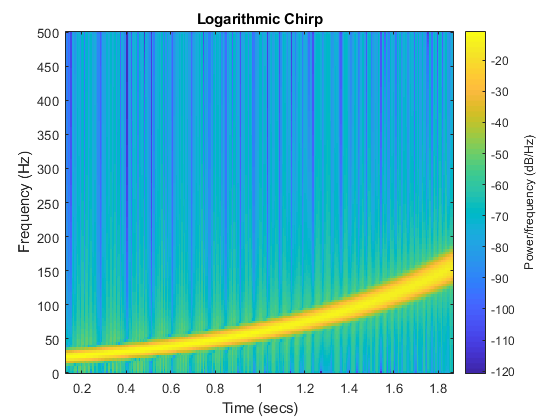
\includegraphics[scale=0.35]{pasta1_figuras/spectrogram1.png}
		\caption{}
	\end{subfigure}
	\hspace*{\fill} % separation between the subfigures
	\begin{subfigure}{0.5\textwidth}
		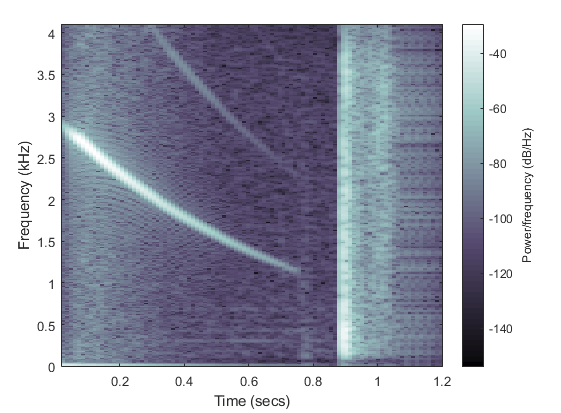
\includegraphics[scale=0.462]{pasta1_figuras/spectrogram4.png}
		\caption{}
	\end{subfigure}

	\begin{subfigure}{0.5\textwidth}
		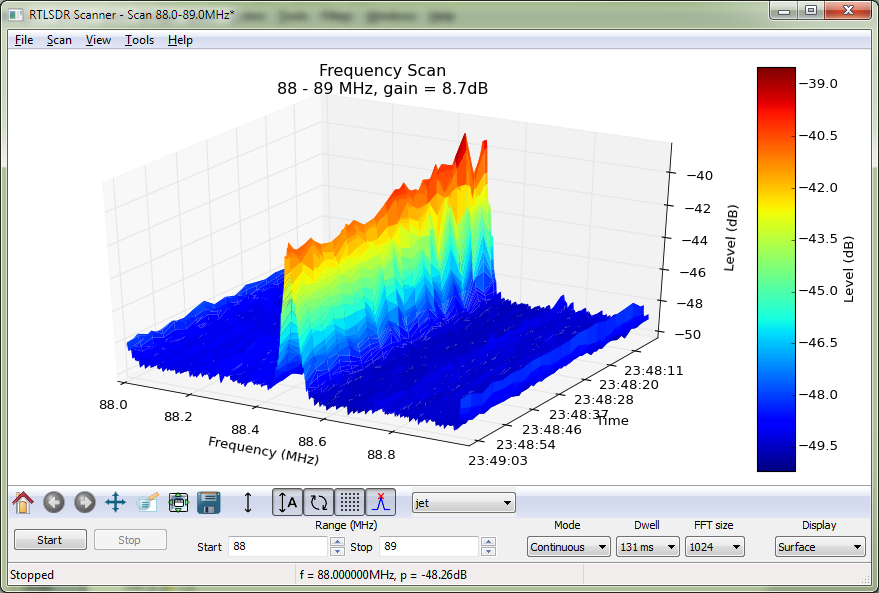
\includegraphics[scale=0.225]{pasta1_figuras/spectrogram2.png}
		\caption{}
	\end{subfigure}
	\hspace*{\fill} % separation between the subfigures
	\begin{subfigure}{0.5\textwidth}
	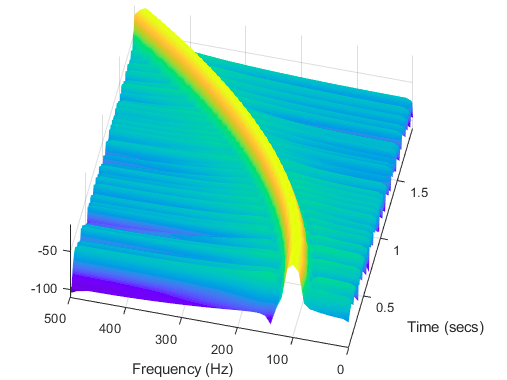
\includegraphics[scale=0.44]{pasta1_figuras/spectrogram3.png}
	\caption{}
	\end{subfigure}
	 \caption{Espectrogramas no MATLAB\rreg} \label{fig-spectrogram}
\end{figure}

O método mais usual para a geração do espectrograma de um sinal é por meio da STFT. Aplicando a técnica, calcula-se a FFT de cada janela do sinal de entrada. Como a saída da FFT pode conter números complexos, computa-se o módulo dos valores de saída da transformada, obtendo-se vários planos de frequências e amplitudes. Por fim, os planos de espectro de cada janela de tempo são colocados lado a lado, formando assim o espectrograma completo.


A equação (\ref{eq-spectrogram}) descreve esse processo com o uso da STFT:

\begin{equation}
	\label{eq-spectrogram}
	spectrogram(x(n), \Delta) = |STFT(x(n),\Delta)|^2
\end{equation}
onde $x(n)$ é o sinal sob análise e $\Delta$ é o tamanho da janela para a STFT.


O MATLAB\rreg fornece o método \textit{spectrogram} para obter, por meio da STFT, o espectrograma de um sinal\cite{mathworks2018spectrogram}. Este método utiliza por padrão o gráfico bidimensional com escala de cores.

%[Detecção de oitavas]
%[Problemas de continuidade]

%\section{Ruído}

%Indicar quais são os quais são os principais fundamentos (algoritmos, paradigmas, teorias) a serem empregados.
%Cada fundamento utilizado deve ser justificado.


% Fim Capítulo
\chapter{Arquiteturas Propostas} \label{cap3}

Neste capítulo são expostas as arquiteturas de redes profundas utilizadas no trabalho.


\section{Visão geral}


\section{Perceptron Multicamadas}
A primeira rede implementada foi o Perceptron Multicamadas. A rede contém: uma camada de entrada, três camadas ocultas e uma camada de saída. A camada de entrada tem o mesmo tamanho da série temporal. As camadas ocultas são compostas por 500 neurônios com a ReLu como função de ativação. A última camada é uma Softmax e contém o número de neurônios igual a quantidade de classes do dataset.

Entre as camadas é utilizada a técnica de \textit{Dropout} com uma taxa de 0.1, 0.2, 0.2 e 0.3, depois da primeira, segunda, terceira e quarta camada respectivamente. Essas taxas determinam uma porcentagem de neurônios que são desativados durante o treinamento em cada época. \textit{Dropout} é uma forma de regularização que ajuda na prevenção do overfitting \cite{dropout2014}. 


\section{Fully Convolutional Networks}

http://principlesofdeeplearning.com/index.php/a-tutorial-on-global-average-pooling/



\chapter{Experimentos} \label{cap4}

Para avaliar o sistema proposto, organizou-se uma bateria de experimentos utilizando a base de dados construída. Os resultados obtidos durante esses experimentos serão comparados com as informações disponíveis a fim de analisar a eficácia do algoritmo de detecção de $f_0$. Neste capítulo, serão relatadas as métricas utilizadas, os objetivos propostos para a experimentação, os resultados obtidos para cada um dos áudios da base de dados e as discussões acerca desses resultados.

\section{Métricas}


Os experimentos consistiram, de modo geral, em submeter os áudios ao sistema desenvolvido, e comparar os resultados obtidos com os arquivos de registros criados manualmente. Para realizar um experimento, deve-se primeiro abrir a interface GUIDE e selecionar, no menu \textit{popup}, o áudio que se deseja analisar. Ao clicar para iniciar o experimento, a interface submete o áudio ao sistema e, com o resultado, plota 4 diferentes gráficos: (i) Gráfico do áudio no tempo, (ii) Espectrograma do áudio, (iii) Saídas do sistema - $f_o$ detectada - no tempo, e (iv) Saídas esperadas - conforme registro manual - sobreposta nas saídas do sistema, ou seja, $f_0$ real sobreposta na $f_0$ detectada. A principal métrica adotada para a avaliação dos experimentos é a comparação visual no último gráfico, que sobrepõe o valor esperado com o valor detectado. Também é possível analisar o desempenho do algoritmo com base no espectrograma. Para um funcionamento ideal do algoritmo, espera-se que os valores detectados estejam sempre juntos com os valores reais.


Outra métrica utilizada para este projeto é o percentual de frequências fundamentais detectadas com sucesso. Para essa métrica, momentos de pausas e silêncios iniciais e finais deveriam ser ignorados, sendo considerado apenas os momentos em que uma nota musical realmente estivesse soando. Outro problema são os arquivos de registro, que não fornecem uma $f_0$ precisa, sendo apenas uma referência para comparação visual. Devido a essa complexidade para se obter a métrica de forma automática, adotou-se um método manual de cálculo desse parâmetro: as detecções erradas serão identificadas e contadas por meio da análise visual do gráfico, sendo considerada errada todas as detecções que estiverem visualmente diferentes da $f_0$ referente à nota soada em cada instante de tempo. Após contabilizar esses erros, faz-se o cálculo percentual de erros em relação ao total de detecções. A métrica de percentual de $f_0$'s detectadas é o inverso da métrica de erro percentual.


Os experimentos foram realizados para cada um dos 4 instrumentos musicais adotados neste projeto, sendo usado para todos eles a referência $196 bpm$ para uma semicolcheia, nota com duração de $\frac{1}{4}$ de tempo de nota.


%Após a geração dos gráficos, a interface de experimentação salva ainda um arquivo de registro com todos os pitch detectados.


% Sobre as estatísticas do experimento.


%Para a análise dos resultados, a saída do sistema foi comparada com o registro original das notas...

\section{Objetivos}

Esta bateria de experimentos tem por objetivo avaliar o desempenho do algoritmo proposto em detectar as frequências fundamentais nos áudios de 4 diferentes instrumentos musicais. Para essa avaliação, espera-se:


\begin{enumerate}
	\item Verificar o percentual de acerto de frequência fundamental, com base no gráfico.
	\item Identificar eventuais problemas de detecção e suas causas.
	\item Discutir acerca da metodologia adotada no desenvolvimento.
\end{enumerate}

\section{Resultados Obtidos}

Nesta seção, os resultados obtidos são expostos a partir dos gráficos gerados e descrição textual.

\subsection{Clarinete}

O clarinete, ou também clarino e clarinete soprano, é um instrumento de sopro. Ele integra o grupo de instrumentos transpositores, ou seja, sua nota soada é diferente da nota escrita na partitura. Isso ocorre pela sua afinação padrão em Bb. As principais características de seu timbre é o som aveludado, encorpado e penetrante, tendo muito brilho nas notas mais agudas. A Figura \ref{fig-clarinete} mostra o clarinete ao lado de sua forma de onda, responsável pelo timbre do instrumento. Foi realizado experimento com os 3 áudios desse instrumento na base de dados: A escala de Bb, a música ``\textit{Agnus Dei}'' e a música tema do \textit{game} ``Super Mário Brós''.

\begin{figure}[h!]
	\centering
	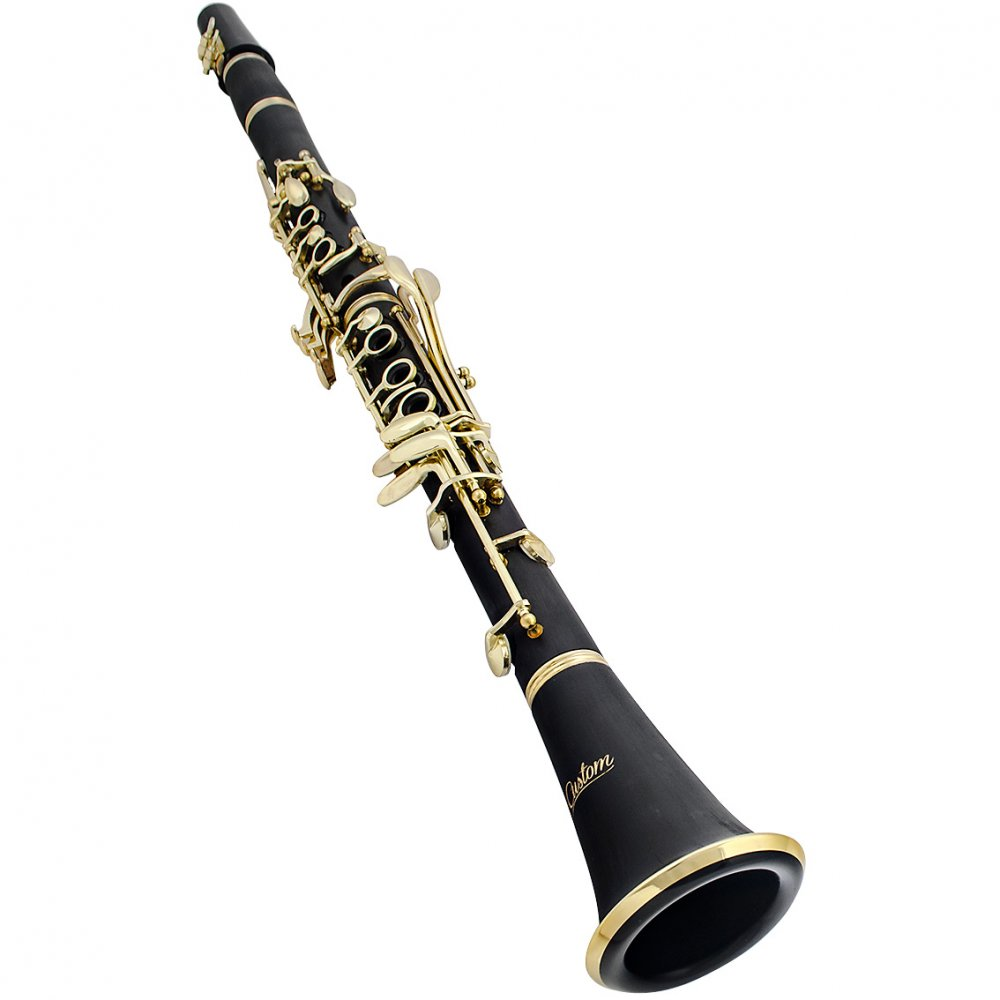
\includegraphics[width=\linewidth/4]{pasta1_figuras/clarinete.jpg}
	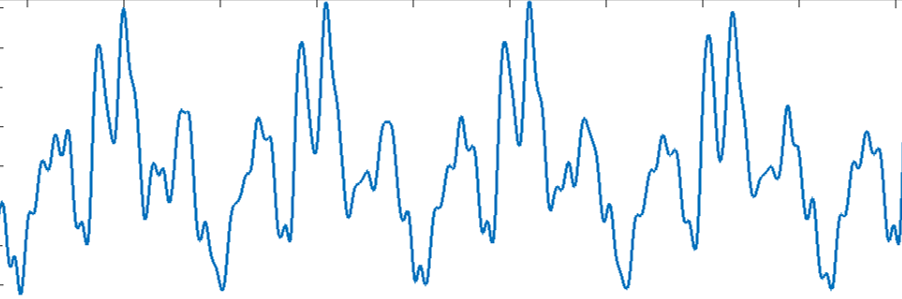
\includegraphics[scale=0.45]{pasta1_figuras/clarinete-timbre.png}
	\caption{Clarinete e sua forma de onda}
	\label{fig-clarinete}
\end{figure}

\subsubsection{Escala: Bb Maior}

O áudio com a escala de Bb Maior no clarinete tem duração de 20 segundos, contando com o tempo inicial sem notas. A Figura \ref{fig-clarinete-escala} exibe a interface gráfica para o experimento com o áudio da escala de Bb Maior.

\begin{figure}
	\centering
	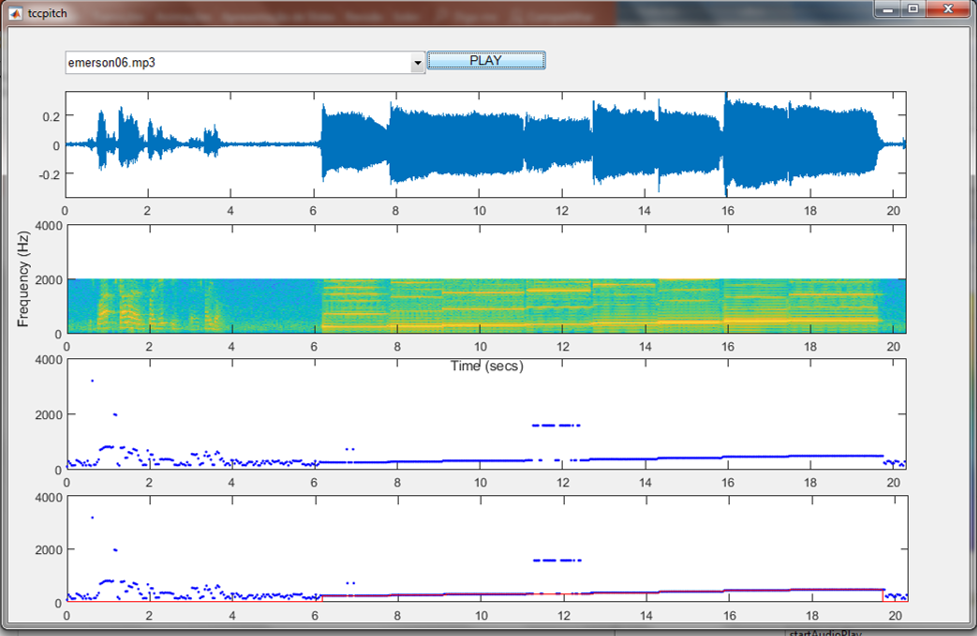
\includegraphics[width=0.75\linewidth]{pasta1_figuras/clarinete-escala.png}
	\caption{Interface de experimentação para áudio "Escala Bb Maior" com clarinete}
	\label{fig-clarinete-escala}
\end{figure}

Os gráficos obtidos no experimento são colocados em separado para melhor visualização das informações. A Figura \ref{fig-clarinete-escala-2} mostra o espectrograma do áudio, a Figura \ref{fig-clarinete-escala-3} exibe as saídas do sistema de detecção de $f_0$, enquanto a Figura \ref{fig-clarinete-escala-4} compara as saídas do sistema de detecção com as frequências esperadas, conforme o arquivo de registros.


Os gráficos demonstram que o sistema obteve sucesso nas detecções de $f_0$, ocorrendo erros em momentos específicos de apenas duas notas, onde detectou-se um harmônico devido ao efeito de ressonância da gravação. Foi calculado um sucesso de 93.4\% nas detecções realizadas para este áudio.

\begin{figure}

\begin{subfigure}{1\textwidth}
	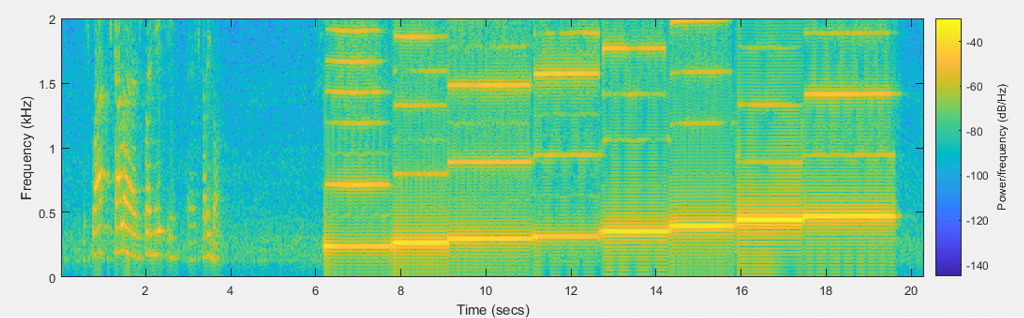
\includegraphics[width=\linewidth]{pasta1_figuras/clarinete-escala-2.png}
	\caption{Espectrograma}
	\label{fig-clarinete-escala-2}
\end{subfigure}
	\hspace*{\fill} % separation between the subfigures
\begin{subfigure}{1\textwidth}
	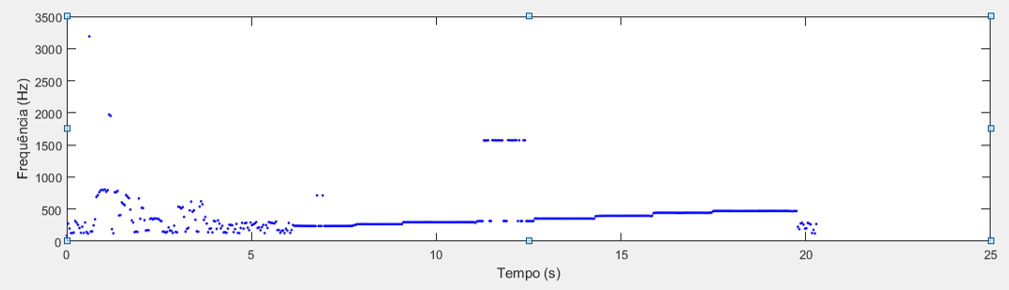
\includegraphics[width=\linewidth]{pasta1_figuras/clarinete-escala-3.png}
	\caption{Detecções de $f_0$}
	\label{fig-clarinete-escala-3}
\end{subfigure}
	\hspace*{\fill} % separation between the subfigures
\begin{subfigure}{1\textwidth}
	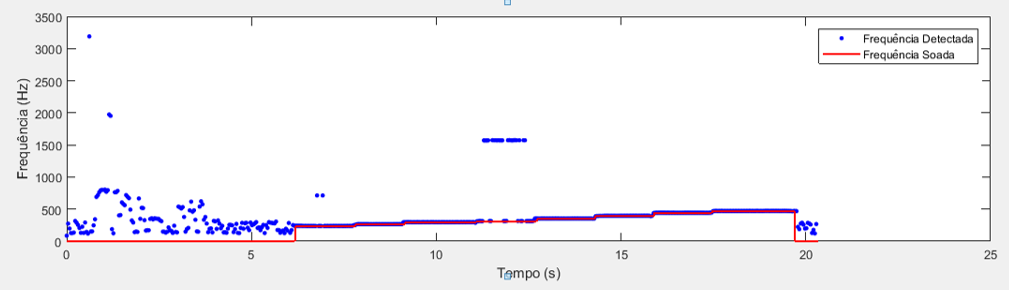
\includegraphics[width=\linewidth]{pasta1_figuras/clarinete-escala-4.png}
	\caption{Comparativo de detecções e registros de $f_0$}
	\label{fig-clarinete-escala-4}
\end{subfigure}
	\caption{Escala de Bb Maior com clarinete}
\end{figure}

\subsubsection{Música: \textit{Agnus Dei}}

O áudio com a música ``\textit{Agnus Dei}'' no clarinete tem duração de 21 segundos. A Figura \ref{fig-clarinete-mario} exibe a interface gráfica para o experimento com esse áudio.

\begin{figure}
	\centering
	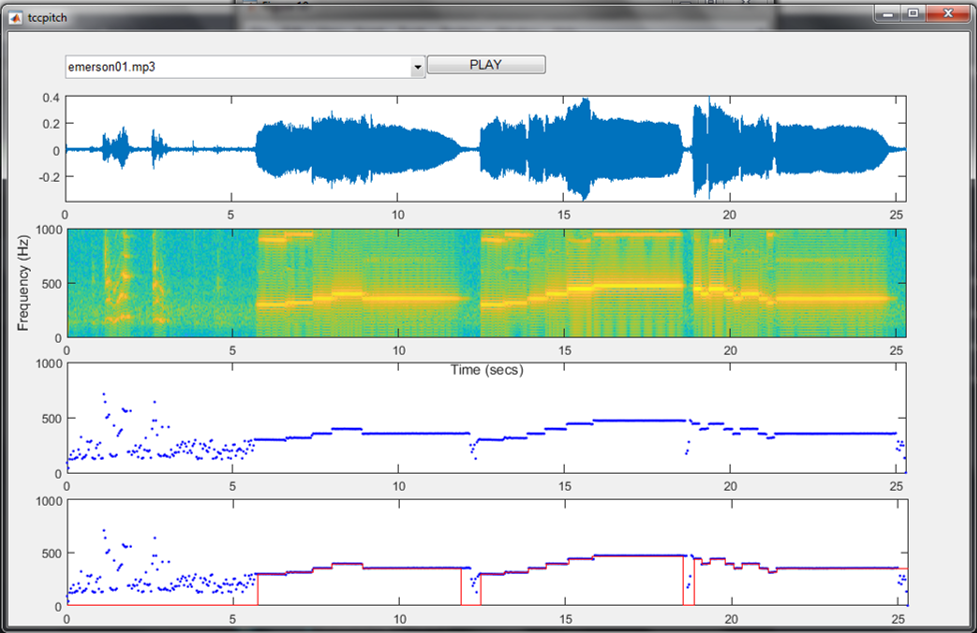
\includegraphics[width=0.75\linewidth]{pasta1_figuras/clarinete-agnusdei.png}
	\caption{Interface de experimentação para áudio da música ``\textit{Agnus Dei}'' com clarinete}
	\label{fig-clarinete-agnusdei}
\end{figure}

Os gráficos obtidos no experimento são colocados em separado para melhor visualização das informações. A Figura \ref{fig-clarinete-mario-2} mostra o espectrograma do áudio, a Figura \ref{fig-clarinete-mario-3} exibe as saídas do sistema de detecção de $f_0$, enquanto a Figura \ref{fig-clarinete-mario-4} compara as saídas do sistema de detecção com as frequências esperadas, conforme o arquivo de registros.


Para esta música, o sistema conseguiu detectar todas as frequências fundamentais, cometendo erro em apenas duas janelas, localizadas em pontos de mudança de nota. O percentual de sucesso na detecção foi de 99.6\%, sendo que os erros podem ser desconsiderados, visto que no instante de alternância entre notas, a janela pode conter mistura de fundamentais da nota anterior com a nova nota que será soada.

\begin{figure}
	\begin{subfigure}{1\textwidth}
		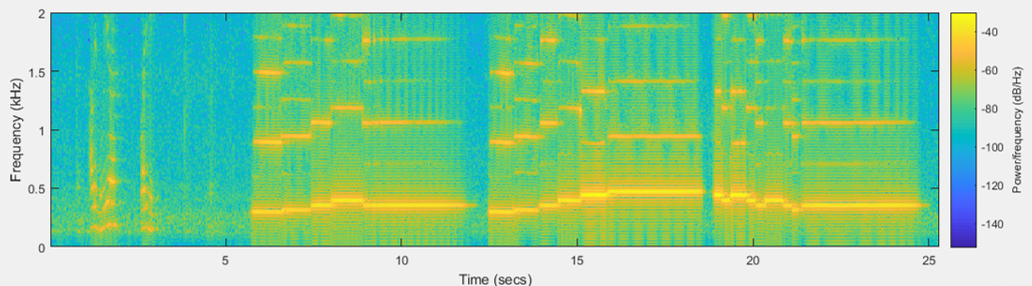
\includegraphics[width=\linewidth]{pasta1_figuras/clarinete-agnusdei-2.png}
		\caption{Espectrograma}
		\label{fig-clarinete-agnusdei-2}
	\end{subfigure}
	\hspace*{\fill} % separation between the subfigures
	\begin{subfigure}{1\textwidth}
		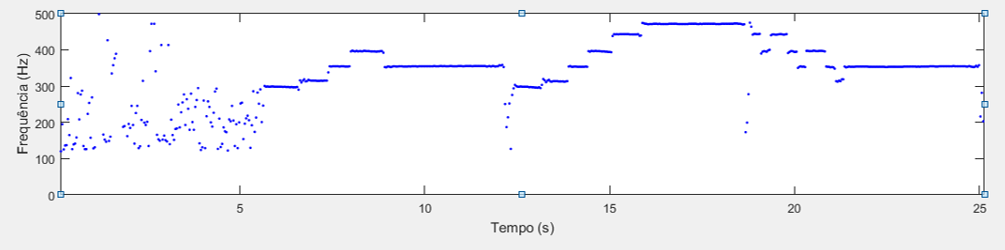
\includegraphics[width=\linewidth]{pasta1_figuras/clarinete-agnusdei-3.png}
		\caption{Detecções de $f_0$}
		\label{fig-clarinete-agnusdei-3}
	\end{subfigure}
	\hspace*{\fill} % separation between the subfigures
	\begin{subfigure}{1\textwidth}
		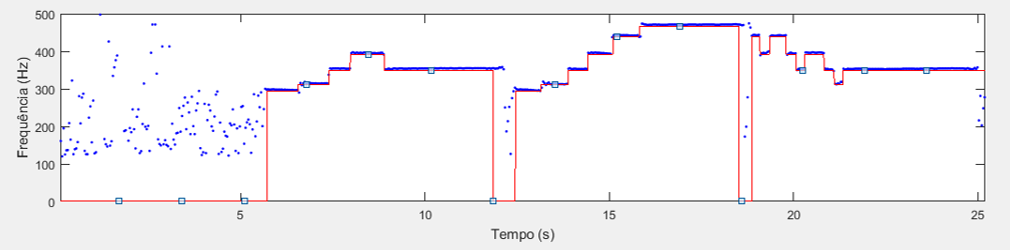
\includegraphics[width=\linewidth]{pasta1_figuras/clarinete-agnusdei-4.png}
		\caption{Comparativo de detecções e registros de $f_0$}
		\label{fig-clarinete-agnusdei-4}
	\end{subfigure}
	\caption{Música ``\textit{Agnus Dei}'' com clarinete}
\end{figure}

\subsubsection{Música: Super Mário Brós}

O áudio com a música tema do \textit{game} ``Super Mário Brós'' no clarinete tem duração de 21 segundos, contando com o tempo inicial sem notas. A Figura \ref{fig-clarinete-mario} exibe a interface gráfica para o experimento com esse áudio.

\begin{figure}
	\centering
	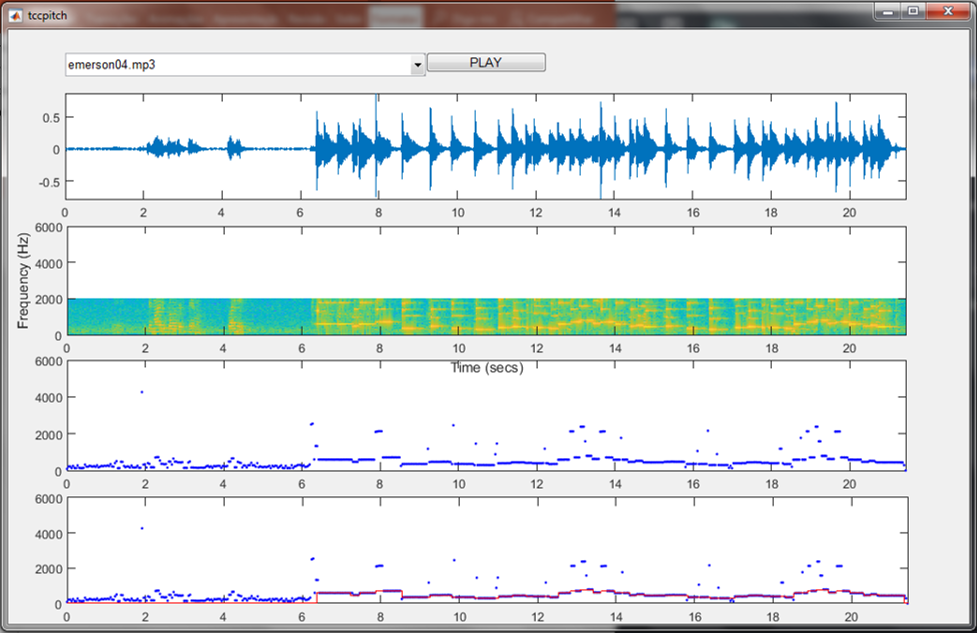
\includegraphics[width=0.75\linewidth]{pasta1_figuras/clarinete-mario.png}
	\caption{Interface de experimentação para áudio da Música ``Super Mário Brós'' com clarinete}
	\label{fig-clarinete-mario}
\end{figure}

Os gráficos obtidos no experimento são colocados em separado para melhor visualização das informações. A Figura \ref{fig-clarinete-mario-2} mostra o espectrograma do áudio, a Figura \ref{fig-clarinete-mario-3} exibe as saídas do sistema de detecção de $f_0$, enquanto a Figura \ref{fig-clarinete-mario-4} compara as saídas do sistema de detecção com as frequências esperadas, conforme o arquivo de registros.


Para este caso, o sistema obteve um bom resultado nas detecções, entretanto, errou em 46 janelas, obtendo um percentual de sucesso nas detecções de 88.2\%. Os erros ocorreram em sua maioria no tempo de subida das notas, e de forma harmônica. Uma característica interessante do clarinete a ser considerada é que, ao soar uma nova nota, se as mãos e a boca do instrumentista não estiverem bem posicionadas no instrumento, percebe-se um leve assobio em um harmônico da nota desejada. Esse efeito ocorre claramente na primeira nota da música tema do ``Super Mário Brós'', e pode ser percebido em mais outra nota durante a execução.

\begin{figure}

\begin{subfigure}{1\textwidth}
	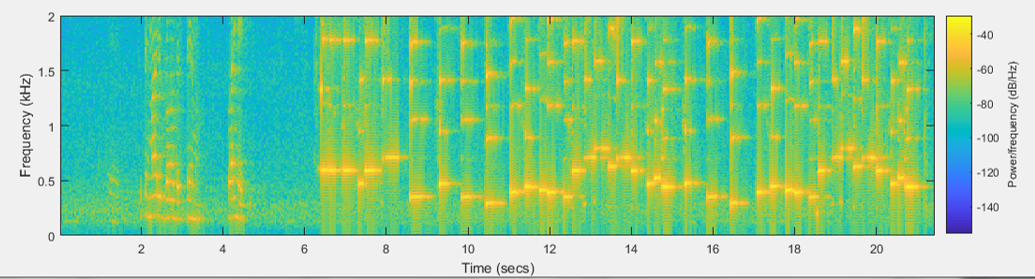
\includegraphics[width=\linewidth]{pasta1_figuras/clarinete-mario-2.png}
	\caption{Espectrograma}
	\label{fig-clarinete-mario-2}
\end{subfigure}

\begin{subfigure}{1\textwidth}
	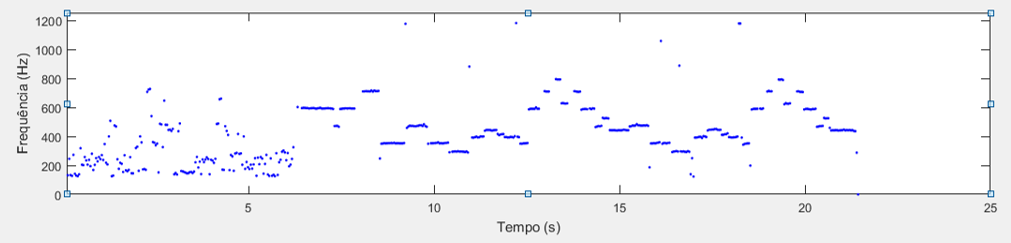
\includegraphics[width=\linewidth]{pasta1_figuras/clarinete-mario-3.png}
	\caption{Detecções de $f_0$}
	\label{fig-clarinete-mario-3}
\end{subfigure}

\begin{subfigure}{1\textwidth}
	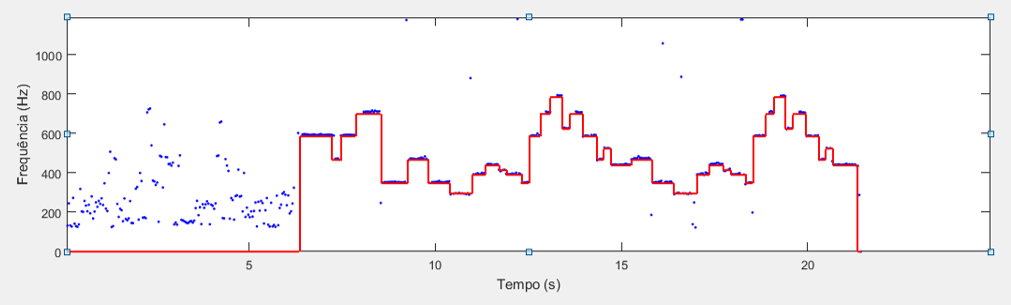
\includegraphics[width=\linewidth]{pasta1_figuras/clarinete-mario-4.png}
	\caption{Comparativo de detecções e registros de $f_0$}
	\label{fig-clarinete-mario-4}
\end{subfigure}
	\caption{Música ``Super Mário Brós'' com clarinete}
\end{figure}



%%%%%
%%
%%
%%%%%

\subsection{Sax Alto}

O Sax Alto também é um instrumento de sopro e, do mesmo modo que o clarinete, está incluso grupo de instrumentos transpositores, ou seja, sua nota soada é diferente da nota escrita na partitura. No caso do sax alto, sua afinação padrão é em Eb. As principais características de seu timbre é o som aveludado, avivado e encorpado. A Figura \ref{fig-sax} mostra o sax alto ao lado de sua forma de onda. Foi realizado experimento com os 3 áudios desse instrumento na base de dados: A escala de Eb, e as músicas ``Deus Cuida de Mim'' e ``\textit{Summertime}''.

\begin{figure}[h!]
	\centering
	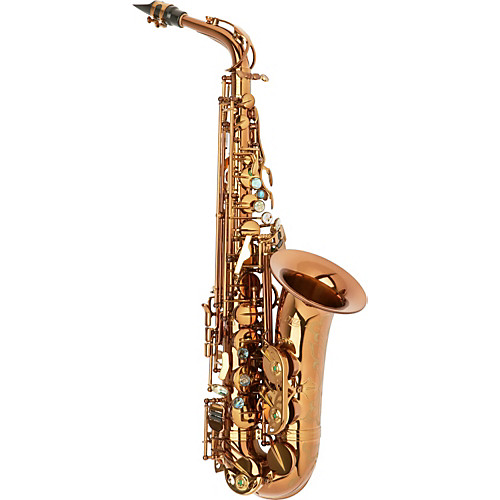
\includegraphics[width=\linewidth/4]{pasta1_figuras/sax.jpg}
	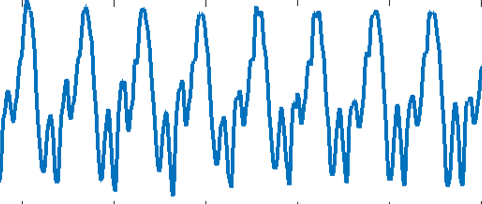
\includegraphics[scale=0.8]{pasta1_figuras/sax-timbre.png}
	\caption{Sax alto e sua forma de onda}
	\label{fig-sax}
\end{figure}

\subsubsection{Escala: Eb Maior}

O áudio com a escala de Eb Maior no sax tem duração de 18 segundos. A Figura \ref{fig-sax-escala} exibe a interface gráfica para o experimento com o áudio da escala de Eb Maior.

\begin{figure}
	\centering
	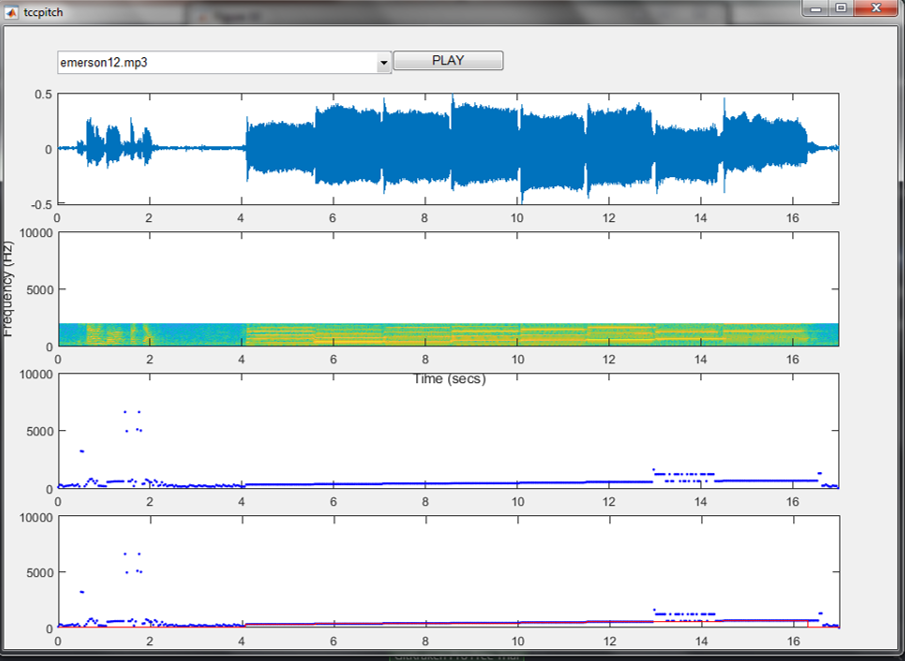
\includegraphics[width=0.75\linewidth]{pasta1_figuras/sax-escala.png}
	\caption{Interface de experimentação para áudio "Escala Eb Maior" com sax alto}
	\label{fig-sax-escala}
\end{figure}

Os gráficos obtidos no experimento são colocados em separado para melhor visualização das informações. A Figura \ref{fig-sax-escala-2} mostra o espectrograma do áudio, a Figura \ref{fig-sax-escala-3} exibe as saídas do sistema de detecção de $f_0$, enquanto a Figura \ref{fig-sax-escala-4} compara as saídas do sistema de detecção com as frequências esperadas, conforme o arquivo de registros.


Para este áudio, o sistema errou a detecção para a nota D5, capturando em mais de 50\% da duração desta nota o harmônico com o dobro da frequência fundamental. Entretanto, não houve nenhum erro nas outras notas. Com isso, o percentual de sucesso na detecção para este áudio foi de 92.8\%, um resultado satisfatório.

\begin{figure}
	
	\begin{subfigure}{1\textwidth}
		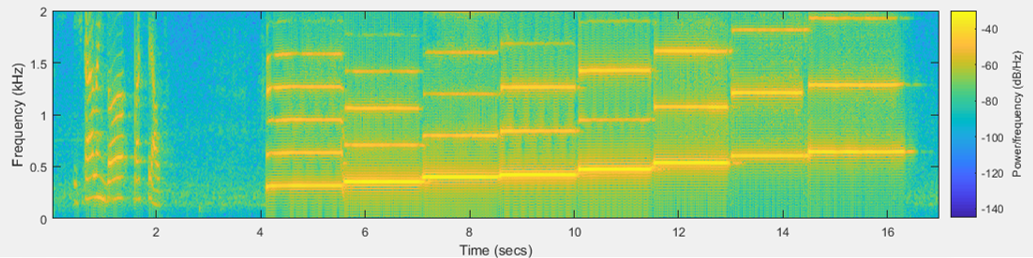
\includegraphics[width=\linewidth]{pasta1_figuras/sax-escala-2.png}
		\caption{Espectrograma}
		\label{fig-sax-escala-2}
	\end{subfigure}
	
	\begin{subfigure}{1\textwidth}
		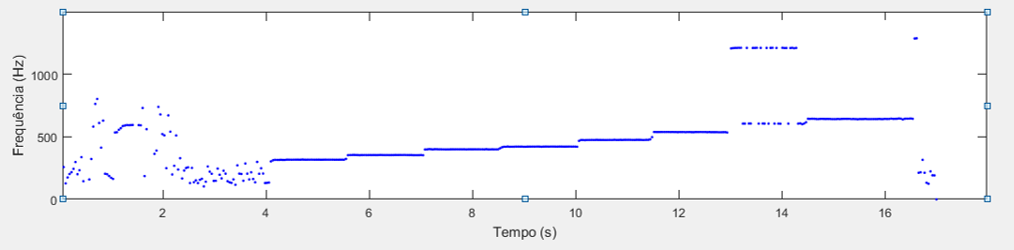
\includegraphics[width=\linewidth]{pasta1_figuras/sax-escala-3.png}
		\caption{Detecções de $f_0$}
		\label{fig-sax-escala-3}
	\end{subfigure}
	
	\begin{subfigure}{1\textwidth}
		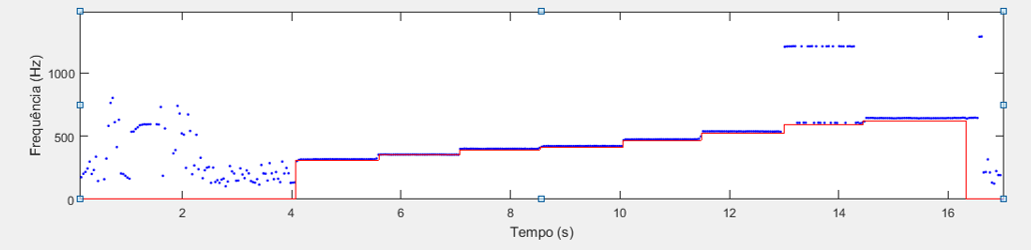
\includegraphics[width=\linewidth]{pasta1_figuras/sax-escala-4.png}
		\caption{Comparativo de detecções e registros de $f_0$}
		\label{fig-sax-escala-4}
	\end{subfigure}
	\caption{Escala Eb Maior com sax alto}
\end{figure}

\subsubsection{Música: Deus Cuida de Mim}

O áudio com a música ``Deus Cuida de Mim'' no sax alto tem duração de 16 segundos. A Figura \ref{fig-sax-Dcm} exibe a interface gráfica para o experimento com esse áudio.

\begin{figure}
	\centering
	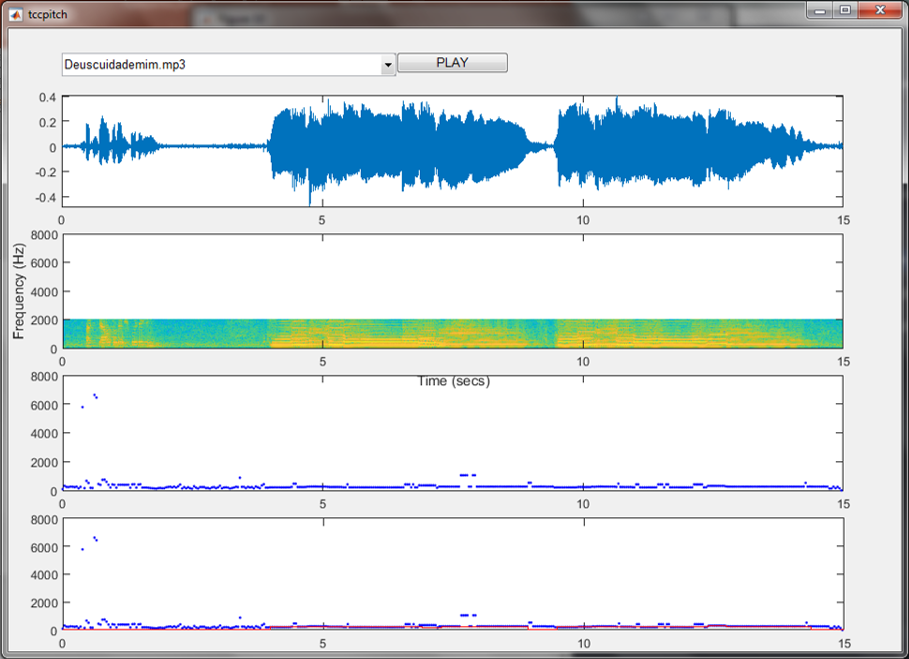
\includegraphics[width=0.75\linewidth]{pasta1_figuras/sax-Dcm.png}
	\caption{Interface de experimentação para áudio da Música ``Deus Cuida de Mim'' com sax alto}
	\label{fig-sax-Dcm}
\end{figure}

Os gráficos obtidos no experimento são colocados em separado para melhor visualização das informações. A Figura \ref{fig-sax-Dcm-2} mostra o espectrograma do áudio, a Figura \ref{fig-sax-Dcm-3} exibe as saídas do sistema de detecção de $f_0$, enquanto a Figura \ref{fig-sax-Dcm-4} compara as saídas do sistema de detecção com as frequências esperadas, conforme o arquivo de registros.


O sistema conseguiu detectar corretamente em 85.9\% das janelas, tendo errado todas as detecções na nota F3. Percebe-se uma real dificuldade em detectar tal nota, pois em ambas as ocorrências dela, detecta-se o harmônico.

\begin{figure}
	
	\begin{subfigure}{1\textwidth}
		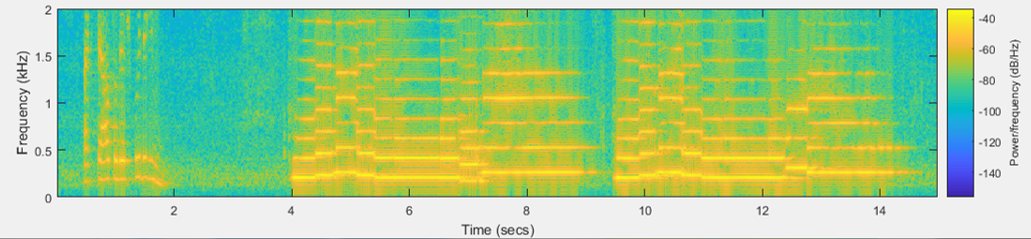
\includegraphics[width=\linewidth]{pasta1_figuras/sax-Dcm-2.png}
		\caption{Espectrograma}
		\label{fig-sax-Dcm-2}
	\end{subfigure}
	\hspace*{\fill} % separation between the subfigures
	\begin{subfigure}{1\textwidth}
		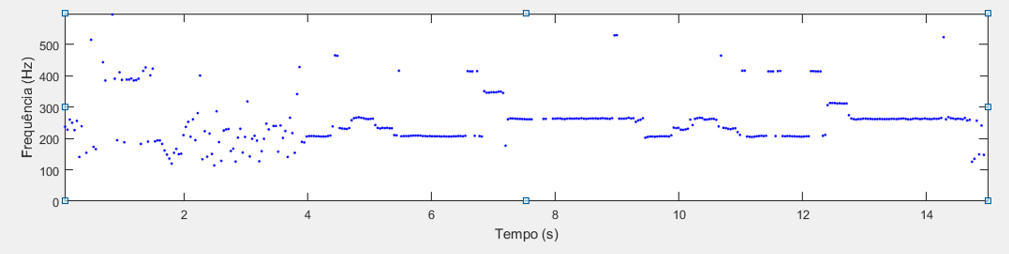
\includegraphics[width=\linewidth]{pasta1_figuras/sax-Dcm-3.png}
		\caption{Detecções de $f_0$}
		\label{fig-sax-Dcm-3}
	\end{subfigure}
	\hspace*{\fill} % separation between the subfigures
	\begin{subfigure}{1\textwidth}
		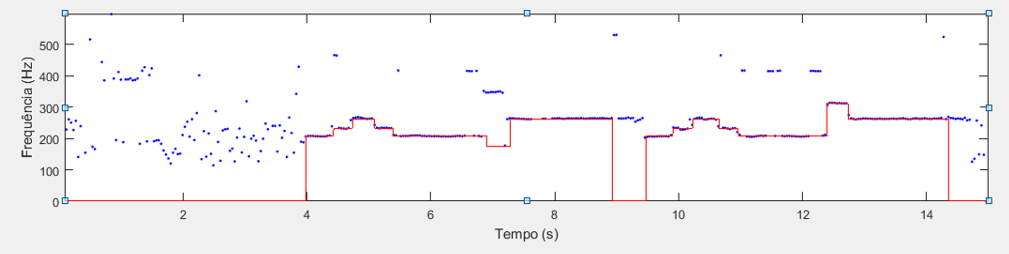
\includegraphics[width=\linewidth]{pasta1_figuras/sax-Dcm-4.png}
		\caption{Comparativo de detecções e registros de $f_0$}
		\label{fig-sax-Dcm-4}
	\end{subfigure}
	\caption{Música ``Deus Cuida de Mim'' no sax alto}
\end{figure}

\subsubsection{Música: \textit{Summertime}}

O áudio com a música ``\textit{Summertime}'' no sax alto tem duração de 29 segundos. A Figura \ref{fig-sax-summer} exibe a interface gráfica para o experimento com esse áudio.

\begin{figure}
	\centering
	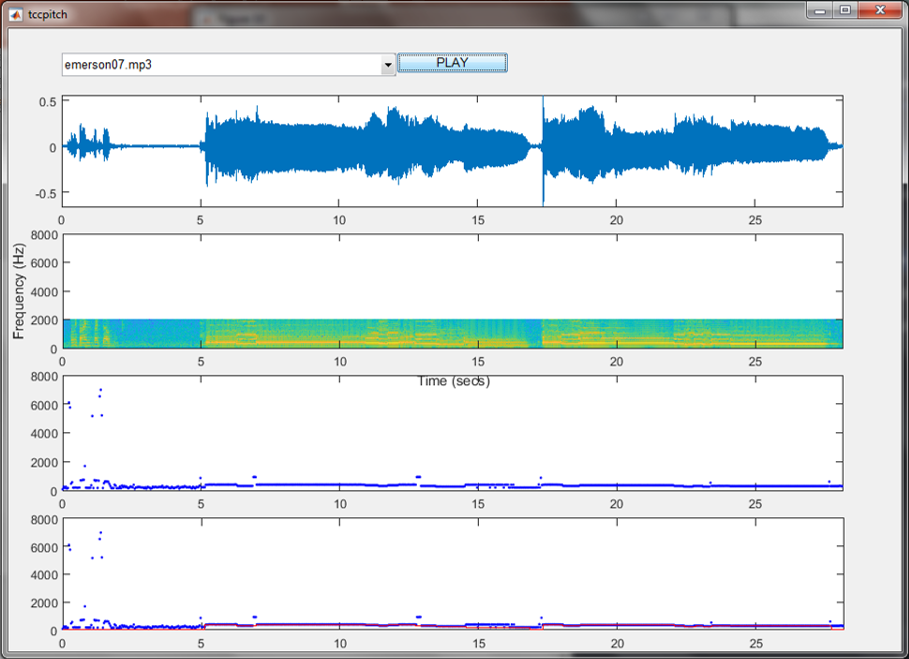
\includegraphics[width=0.75\linewidth]{pasta1_figuras/sax-summer.png}
	\caption{Interface de experimentação para áudio da música ``\textit{Summertime}'' com sax alto}
	\label{fig-sax-summer}
\end{figure}

Os gráficos obtidos no experimento são colocados em separado para melhor visualização das informações. A Figura \ref{fig-sax-summer-2} mostra o espectrograma do áudio, a Figura \ref{fig-sax-summer-3} exibe as saídas do sistema de detecção de $f_0$, enquanto a Figura \ref{fig-sax-summer-4} compara as saídas do sistema de detecção com as frequências esperadas, conforme o arquivo de registros.


Para este áudio, o sistema também errou em mais de 50\% da duração de uma das notas, dessa vez G3, única nota da 3ª escala na música. Entretanto, as detecções nas demais notas, todas da 4ª escala, obtiveram mínimos erros, de modo que a taxa de sucesso nas detecções foi de 91.5\%. Com este áudio, ficou evidente que há uma dificuldade para que o sistema consiga detectar frequências fundamentais para notas abaixo de 200Hz no saxofone alto.


\begin{figure}
	
	\begin{subfigure}{1\textwidth}
		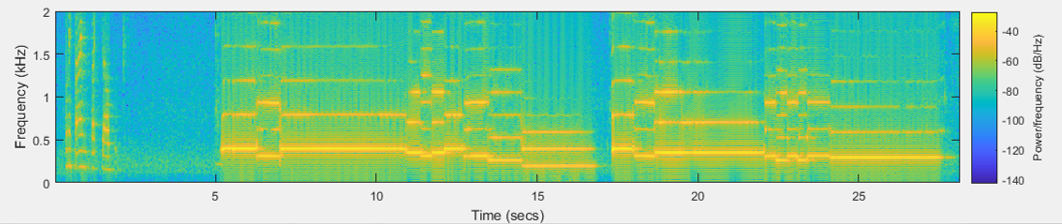
\includegraphics[width=\linewidth]{pasta1_figuras/sax-summer-2.png}
		\caption{Espectrograma}
		\label{fig-sax-summer-2}
	\end{subfigure}
	
	\begin{subfigure}{1\textwidth}
		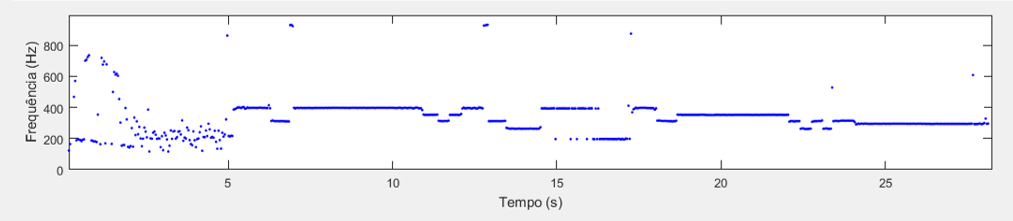
\includegraphics[width=\linewidth]{pasta1_figuras/sax-summer-3.png}
		\caption{Detecções de $f_0$}
		\label{fig-sax-summer-3}
	\end{subfigure}
	
	\begin{subfigure}{1\textwidth}
		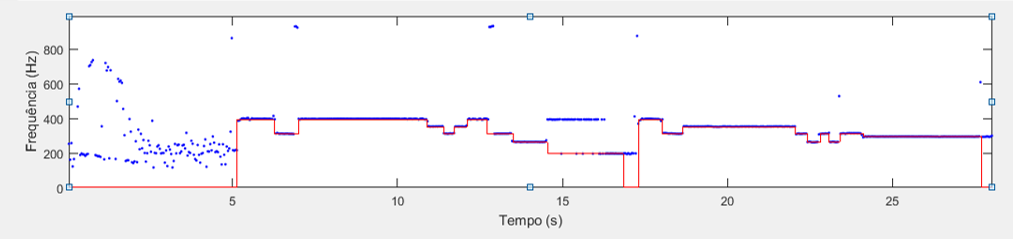
\includegraphics[width=\linewidth]{pasta1_figuras/sax-summer-4.png}
		\caption{Comparativo de detecções e registros de $f_0$}
		\label{fig-sax-summer-4}
	\end{subfigure}
	\caption{Audio da música ``\textit{Summertime}'' no sax alto}
\end{figure}


%%%%%%
%%%
%%%
%%%%%%


\subsection{Piano Eletrônico}

O piano é um instrumento de corda percussivas, entretanto, o piano eletrônico tem o papel de facilitar o uso do piano, de modo que torna-se cada vez mais raro encontrar um piano acústico sendo usado. O piano eletrônico busca imitar o som do piano acústico e, embora não seja perfeitamente igual, já alcança uma boa semelhança. A Figura \ref{fig-piano} mostra o piano eletrônico ao lado de sua forma de onda, responsável pelo timbre do instrumento.

\begin{figure} [h!]
	\centering
	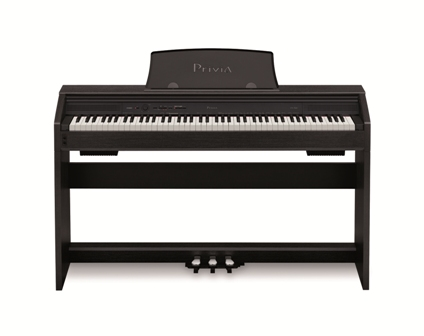
\includegraphics[width=\linewidth/4]{pasta1_figuras/piano.png}
	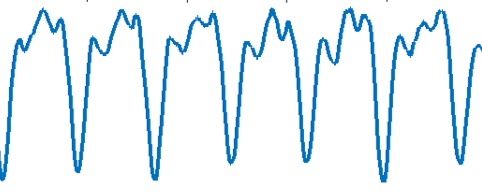
\includegraphics[scale=0.8]{pasta1_figuras/piano-timbre.png}
	\caption{Piano e sua forma de onda}
	\label{fig-piano}
\end{figure}

\subsubsection{Escala: C Maior}

O áudio com a escala de C Maior no piano tem duração de 12 segundos. A Figura \ref{fig-piano-escala} exibe a interface gráfica para o experimento com o áudio da escala de C Maior no piano eletrônico.

\begin{figure}
	\centering
	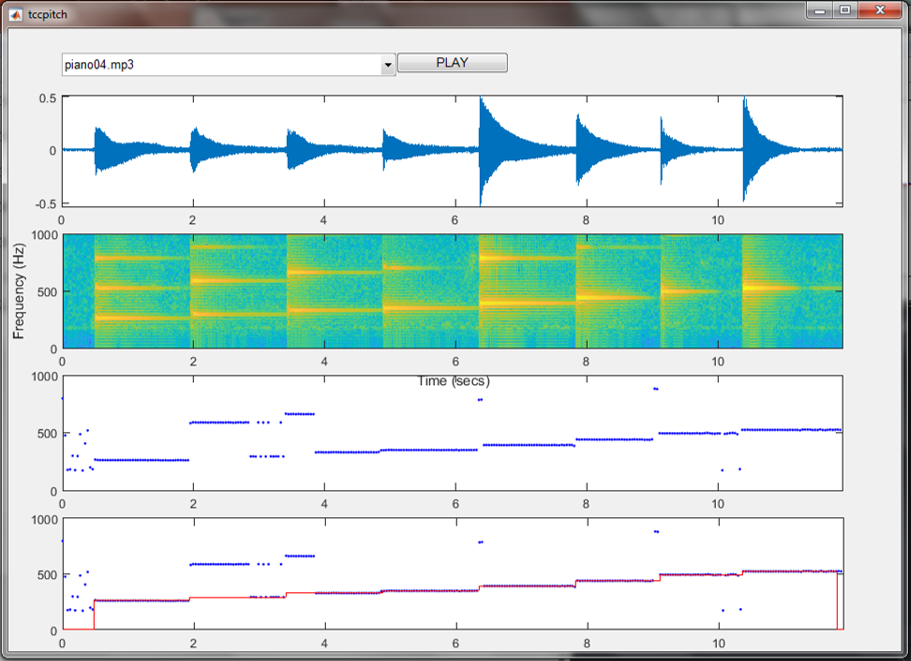
\includegraphics[width=0.75\linewidth]{pasta1_figuras/piano-escala.png}
	\caption{Interface de experimentação para áudio da escala C Maior com piano eletrônico}
	\label{fig-piano-escala}
\end{figure}

Os gráficos obtidos no experimento são colocados em separado para melhor visualização das informações. A Figura \ref{fig-piano-escala-2} mostra o espectrograma do áudio, a Figura \ref{fig-piano-escala-3} exibe as saídas do sistema de detecção de $f_0$, enquanto a Figura \ref{fig-piano-escala-4} compara as saídas do sistema de detecção com as frequências esperadas, conforme o arquivo de registros.


Para a escala de C Maior, o sistema obteve percentual de sucesso nas detecções de 85.1\%. As notas D4 e E4 foram as que mais tiveram erros, tendo suas harmônicas detectadas no dobro da $f_0$ real. Nas demais notas, o sistema conseguiu trabalhar bem.

\begin{figure}
	
	\begin{subfigure}{1\textwidth}
		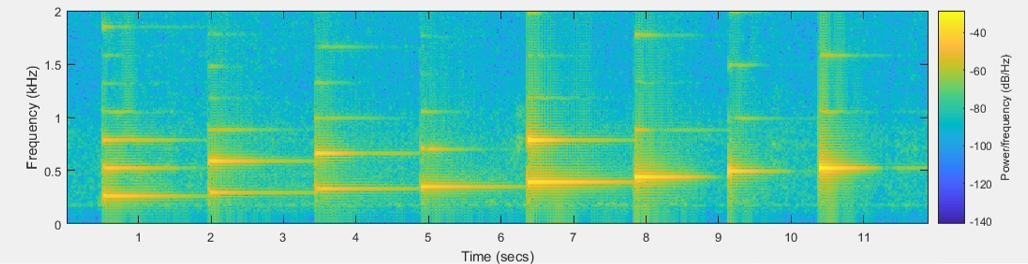
\includegraphics[width=\linewidth]{pasta1_figuras/piano-escala-2.png}
		\caption{Espectrograma}
		\label{fig-piano-escala-2}
	\end{subfigure}
	
	\begin{subfigure}{1\textwidth}
		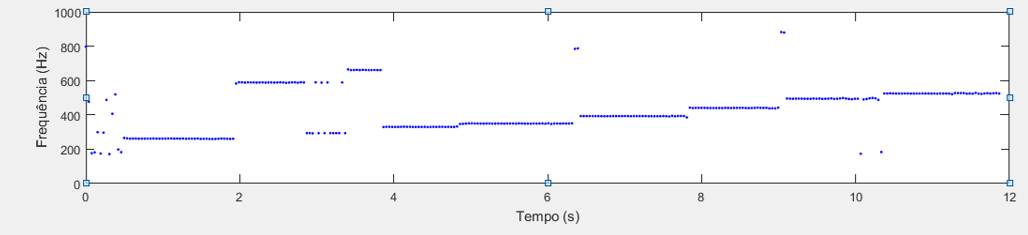
\includegraphics[width=\linewidth]{pasta1_figuras/piano-escala-3.png}
		\caption{Detecções de $f_0$}
		\label{fig-piano-escala-3}
	\end{subfigure}
	
	\begin{subfigure}{1\textwidth}
		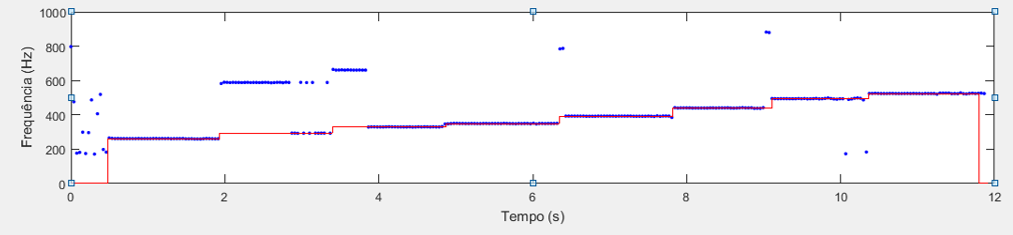
\includegraphics[width=\linewidth]{pasta1_figuras/piano-escala-4.png}
		\caption{Comparativo de detecções e registros de $f_0$}
		\label{fig-piano-escala-4}
	\end{subfigure}
	\caption{Escala de C Maior no piano eletrônico}
\end{figure}

\subsubsection{Música: Eu Navegarei}

O áudio com a música ``Eu Navegarei'' no piano tem duração de 22 segundos. A Figura \ref{fig-piano-navegarei} exibe a interface gráfica para o experimento com esse áudio.

\begin{figure}
	\centering
	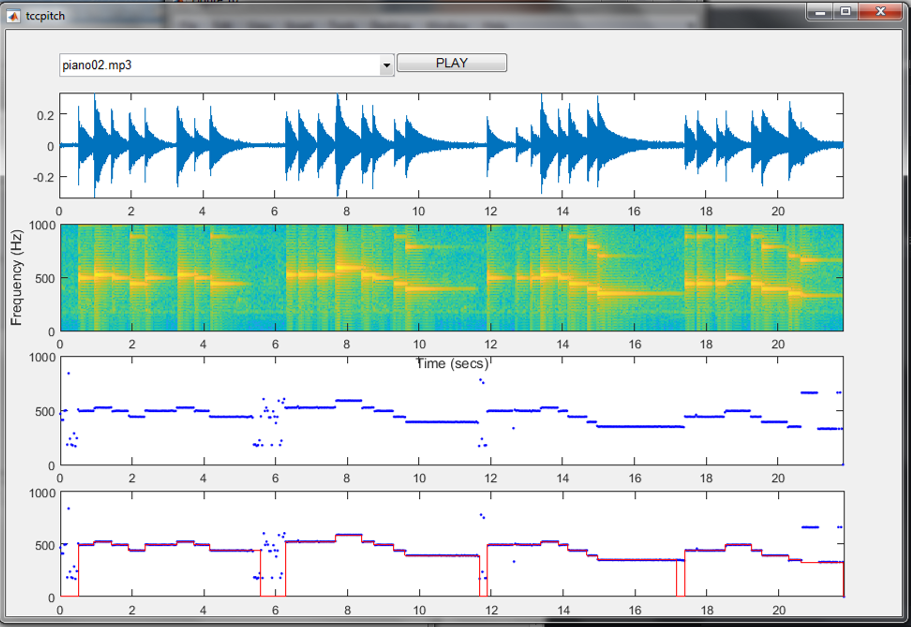
\includegraphics[width=0.75\linewidth]{pasta1_figuras/piano-navegarei.png}
	\caption{Interface de experimentação para áudio da música ``Eu Navegarei'' com piano eletrônico}
	\label{fig-piano-navegarei}
\end{figure}

Os gráficos obtidos no experimento são colocados em separado para melhor visualização das informações. A Figura \ref{fig-piano-navegarei-2} mostra o espectrograma do áudio, a Figura \ref{fig-piano-navegarei-3} exibe as saídas do sistema de detecção de $f_0$, enquanto a Figura \ref{fig-piano-navegarei-4} compara as saídas do sistema de detecção com as frequências esperadas, conforme o arquivo de registros.


Para este áudio, o sistema obteve sucesso em 97\% das janelas analisadas. A maior parte dos 3\% de erros foram durante a execução de uma nota E4, repetindo o problema detectado no áudio da escala de C Maior. Mesmo assim, o sistema alcançou um resultado muito satisfatório para esse experimento

\begin{figure}
	
	\begin{subfigure}{1\textwidth}
		\includegraphics[width=\linewidth]{pasta1_figuras/piano-navegarei-2.png}
		\caption{Espectrograma}
		\label{fig-piano-navegarei-2}
	\end{subfigure}
	\hspace*{\fill} % separation between the subfigures
	\begin{subfigure}{1\textwidth}
		\includegraphics[width=\linewidth]{pasta1_figuras/piano-navegarei-3.png}
		\caption{Detecções de $f_0$}
		\label{fig-piano-navegarei-3}
	\end{subfigure}
	\hspace*{\fill} % separation between the subfigures
	\begin{subfigure}{1\textwidth}
		\includegraphics[width=\linewidth]{pasta1_figuras/piano-navegarei-4.png}
		\caption{Comparativo de detecções e registros de $f_0$}
		\label{fig-piano-navegarei-4}
	\end{subfigure}
	\caption{Áudio da música ``Eu Navegarei'' tocado com piano eletrônico}
\end{figure}

\subsubsection{Música: \textit{Skyfall}}

O áudio com a música ``\textit{Skyfall}'' no piano tem duração de 12 segundos. A Figura \ref{fig-piano-skyfall} exibe a interface gráfica para o experimento com esse áudio.

\begin{figure}
	\centering
	\includegraphics[width=0.75\linewidth]{pasta1_figuras/piano-skyfall.png}
	\caption{Interface de experimentação para áudio da música ``\textit{Skyfall}'' com piano}
	\label{fig-piano-skyfall}
\end{figure}

Os gráficos obtidos no experimento são colocados em separado para melhor visualização das informações. A Figura \ref{fig-piano-skyfall-2} mostra o espectrograma do áudio, a Figura \ref{fig-piano-skyfall-3} exibe as saídas do sistema de detecção de $f_0$, enquanto a Figura \ref{fig-piano-skyfall-4} compara as saídas do sistema de detecção com as frequências esperadas, conforme o arquivo de registros.


Para o áudio ``\textit{Skyfall}'', o sistema teve dois tipos de erros principais: O primeiro refere-se ao problema para detectar Eb4, pois em todos os experimentos com piano eletrônico, o sistema demonstrou uma grande dificuldade em detectar as fundamentais relativas as notas D4, Eb4 e E4, entre 290Hz e 330Hz. O segundo problema esteve relacionado ao  decaimento da nota. Neste áudio, o sistema obteve 79.5\% de taxa de sucesso nas detecções, um valor bem abaixo da média alcançada entre os instrumentos de sopro.

\begin{figure}
	
	\begin{subfigure}{1\textwidth}
		\includegraphics[width=\linewidth]{pasta1_figuras/piano-skyfall-2.png}
		\caption{Espectrograma}
		\label{fig-piano-skyfall-2}
	\end{subfigure}
	
	\begin{subfigure}{1\textwidth}
		\includegraphics[width=\linewidth]{pasta1_figuras/piano-skyfall-3.png}
		\caption{Detecções de $f_0$}
		\label{fig-piano-skyfall-3}
	\end{subfigure}
	
	\begin{subfigure}{1\textwidth}
		\includegraphics[width=\linewidth]{pasta1_figuras/piano-skyfall-4.png}
		\caption{Comparativo de detecções e registros de $f_0$}
		\label{fig-piano-skyfall-4}
	\end{subfigure}
	\caption{Música ``\textit{Skyfall}'' tocada no piano}
\end{figure}


%%%%%%
%%%
%%%
%%%%%%

\subsection{Violão}

O violão é um instrumento de corda. A Figura \ref{fig-violao} mostra o violão ao lado de sua forma de onda.

\begin{figure}[h!]
	\centering
	\includegraphics[width=\linewidth/4]{pasta1_figuras/violao.jpg}
	\includegraphics[scale=0.8]{pasta1_figuras/violao-timbre.png}
	\caption{Violão e sua forma de onda}
	\label{fig-violao}
\end{figure}

\subsubsection{Escala: C Maior}

O áudio com a escala de C Maior no violão tem duração de 17 segundos, contando com o tempo inicial de silêncio. A Figura \ref{fig-violao-escala} exibe a interface gráfica para o experimento com o áudio da escala de C Maior tocada pelo violão.

\begin{figure}
	\centering
	\includegraphics[width=0.75\linewidth]{pasta1_figuras/violao-escala.png}
	\caption{Interface de experimentação para áudio da escala de C Maior com violão}
	\label{fig-violao-escala}
\end{figure}

Os gráficos obtidos no experimento são colocados em separado para melhor visualização das informações. A Figura \ref{fig-violao-escala-2} mostra o espectrograma do áudio, a Figura \ref{fig-violao-escala-3} exibe as saídas do sistema de detecção de $f_0$, enquanto a Figura \ref{fig-violao-escala-4} compara as saídas do sistema de detecção com as frequências esperadas, conforme o arquivo de registros.


Para este áudio, o sistema apresentou o pior resultado, tendo 46.3\% de sucesso nas detecções. Somente as notas C3, A3 e C4 foram detectadas corretamente, enquanto todas as outras foram detectas no harmônico com dobro de $f_0$. A principal característica a ser considerada nessa questão é o funcionamento físico do violão, que amplia o som da vibração de suas cordas através de sua caixa de ressonância. Sendo assim, é comum que o fenômeno da ressonância aconteça, o que atrapalha a performance do sistema. 

\begin{figure}
	
	\begin{subfigure}{1\textwidth}
		\includegraphics[width=\linewidth]{pasta1_figuras/violao-escala-2.png}
		\caption{Espectrograma}
		\label{fig-violao-escala-2}
	\end{subfigure}
	
	\begin{subfigure}{1\textwidth}
		\includegraphics[width=\linewidth]{pasta1_figuras/violao-escala-3.png}
		\caption{Detecções de $f_0$}
		\label{fig-violao-escala-3}
	\end{subfigure}
	
	\begin{subfigure}{1\textwidth}
		\includegraphics[width=\linewidth]{pasta1_figuras/violao-escala-4.png}
		\caption{Comparativo de detecções e registros de $f_0$}
		\label{fig-violao-escala-4}
	\end{subfigure}
	\caption{Escala de C Maior no violão}
\end{figure}

\subsubsection{Música: Nona Sinfonia}

O áudio com a música ``Nona Sinfonia'' no violão tem duração de 15 segundos, contando com o tempo inicial sem notas. A Figura \ref{fig-violao-nona} exibe a interface gráfica para o experimento com esse áudio.

\begin{figure}
	\centering
	\includegraphics[width=0.75\linewidth]{pasta1_figuras/violao-nona.png}
	\caption{Interface de experimentação para áudio da música ``Nona Sinfonia'' com violão}
	\label{fig-violao-nona}
\end{figure}

Os gráficos obtidos no experimento são colocados em separado para melhor visualização das informações. A Figura \ref{fig-violao-nona-2} mostra o espectrograma do áudio, a Figura \ref{fig-violao-nona-3} exibe as saídas do sistema de detecção de $f_0$, enquanto a Figura \ref{fig-violao-nona-4} compara as saídas do sistema de detecção com as frequências esperadas, conforme o arquivo de registros.


Para este áudio, a detecção obteve taxa de 72.4\% de sucesso nas detecções. Somente a nota G3 que não foi detectada, tendo sido apontado o harmônico da $f_0$. Esse resultado evidencia que a dificuldade com sons mais graves acontece em todos os instrumentos, sendo difícil diferenciar qual o harmônico fundamental.

\begin{figure}
	
	\begin{subfigure}{1\textwidth}
		\includegraphics[width=\linewidth]{pasta1_figuras/violao-nona-2.png}
		\caption{Espectrograma}
		\label{fig-violao-nona-2}
	\end{subfigure}
	\hspace*{\fill} % separation between the subfigures
	\begin{subfigure}{1\textwidth}
		\includegraphics[width=\linewidth]{pasta1_figuras/violao-nona-3.png}
		\caption{Detecções de $f_0$}
		\label{fig-violao-nona-3}
	\end{subfigure}
	\hspace*{\fill} % separation between the subfigures
	\begin{subfigure}{1\textwidth}
		\includegraphics[width=\linewidth]{pasta1_figuras/violao-nona-4.png}
		\caption{Comparativo de detecções e registros de $f_0$}
		\label{fig-violao-nona-4}
	\end{subfigure}
		\caption{Música ``Nona Sinfonia'' tocada no violão.}
\end{figure}

\subsubsection{Música: Deus de Abraão}

Por fim, o último áudio a ser analisado foi a música ``Deus de Abraão'' no violão, que tem duração de 22 segundos, contando com o tempo inicial de silêncio. A Figura \ref{fig-violao-002CC} exibe a interface gráfica para o experimento com esse áudio.

\begin{figure}
	\centering
	\includegraphics[width=0.75\linewidth]{pasta1_figuras/violao-002CC.png}
	\caption{Interface de experimentação para áudio da música ``Deus de Abraão'' com violão}
	\label{fig-violao-002CC}
\end{figure}

Os gráficos obtidos no experimento são colocados em separado para melhor visualização das informações. A Figura \ref{fig-violao-002CC-2} mostra o espectrograma do áudio, a Figura \ref{fig-violao-002CC-3} exibe as saídas do sistema de detecção de $f_0$, enquanto a Figura \ref{fig-violao-002CC-4} compara as saídas do sistema de detecção com as frequências esperadas, conforme o arquivo de registros.


Os resultados para esse áudio foram bem acima do esperado, alcançando na detecção de $f_0$, para notas de violão, a taxa de sucesso de 92.6\%. O sucesso se deve principalmente ao uso de notas mais agudas, em maioria da 4ª oitava. Nesse experimento, os erros ocorreram em sua maioria nas 2 notas mais graves, pertencentes a 3ª oitava (F\#3 e B3). Deste modo, fica evidente que o sistema apresenta bons resultados para sons mais agudos, e tem maior dificuldade para discernir sons mais graves.

\begin{figure}
	
	\begin{subfigure}{1\textwidth}
		\includegraphics[width=\linewidth]{pasta1_figuras/violao-002CC-2.png}
		\caption{Espectrograma}
		\label{fig-violao-002CC-2}
	\end{subfigure}
	
	\begin{subfigure}{1\textwidth}
		\includegraphics[width=\linewidth]{pasta1_figuras/violao-002CC-3.png}
		\caption{Detecções de $f_0$}
		\label{fig-violao-002CC-3}
	\end{subfigure}
	
	\begin{subfigure}{1\textwidth}
		\includegraphics[width=\linewidth]{pasta1_figuras/violao-002CC-4.png}
		\caption{Comparativo de detecções e registros de $f_0$}
		\label{fig-violao-002CC-4}
	\end{subfigure}
	\caption{Música ``Deus de Abraão'' tocada no violão.}
\end{figure}



\section{Discussões}

O sistema alcançou resultados satisfatórios, visto que detectou com sucesso um percentual de cerca de 85\% das frequências fundamentais. Entre os instrumentos de sopro, o percentual médio de sucesso ultrapassou os 90\%. Em compensação, percebeu-se que o sistema ainda é deficiente em melodias graves, principalmente para instrumentos de corda. A Tabela \ref{table-compare-songs} exibe as taxas de sucesso obtidas em cada áudio. Os erros nas detecções estiveram em sua maioria relacionados a dificuldade do sistema em detectar fundamentais em notas muito graves, e em outros casos, os erros eram em função de não sustentação da nota ou ruídos de execução. Muitos desses erros podem ser evitados se o sistema for combinado a algum método estatístico de tratamento que identifique a continuidade de uma nota. Entretanto, torna-se um verdadeiro desafio garantir a detecção para notas com efeito de ressonância.

\begin{table}[h]
	\centering
	\caption{Comparativo entre os áudios} 	\label{table-compare-songs}
	\begin{tabular}{|c|c|c|}
		\hline
		\textbf{INSTRUMENTO}       & \textbf{ÁUDIO} & \multicolumn{1}{c|}{\textbf{\begin{tabular}[c]{@{}c@{}}SUCESSO NAS\\ DETECÇÕES\end{tabular}}} \\ \hline
		\multirow{3}{*}{CLARINETE} & Escala - Bb Maior & 93.4\%         \\ \cline{2-3} 
		& Música - \textit{Agnus Dei}  & 99.6\%       \\ \cline{2-3} 
		& Música - Super Mário Brós & 88.2\% \\ \hline
		\multirow{3}{*}{SAX ALTO}  & Escala - Bb Maior  & 92.8\%         \\ \cline{2-3} 
		& Música - Deus Cuida de Mim & 85.9\% \\ \cline{2-3} 
		& Música - \textit{Summertime}   & 91.5\%     \\ \hline
		\multirow{3}{*}{PIANO ELETRÔNICO}     & Escala - C Maior    & 85.1\%       \\ \cline{2-3} 
		& Música - Eu Navegarei   & 97.0\%   \\ \cline{2-3} 
		& Música - \textit{Skyfall}    & 79.5\%     \\ \hline
		\multirow{3}{*}{VIOLÃO}    & Escala - C Maior    & 46.4\%       \\ \cline{2-3} 
		& Música - Nona Sinfonia  & 72.4\%   \\ \cline{2-3} 
		& Música - Ao Deus de Abraão & 92.6\% \\ \hline
	\end{tabular}
\end{table}

O método de detecção de $f_0$ buscando a frequência de maior amplitude, por meio da STFT, é trivialmente falho na ocorrência de ressonância, visto que o efeito de ressonância consiste na superação da amplitude da fundamental por um harmônico em frequência diferente. Diante desse problema, torna-se necessário combinar o método proposto com outros métodos que busquem identificar o efeito de ressonância, de modo a tratar os erros causados por esse efeito. Neste sentido, o sistema implementado apenas da forma como foi proposto não está apto para a detecção de fundamentais em contextos que apresentem o efeito de ressonância. De todo modo, as fundamentais detectadas em 99\% das vezes eram suficientes para fornecer informações da nota soada, divergindo apenas para identificar a oitava a qual essa nota pertence.


A metodologia adotada para a implementação desse projeto mostrou-se de grande potencial, podendo ser evoluída para um sistema mais robusto e com menor sensibilidade ao efeito de ressonância. O ambiente montado para a experimentação também demonstrou ser prático e de fácil manutenção, permitindo que o ritmo de experimentação seja satisfatório. A base de dados foi utilizada com sucesso, e permitiu a verificação de diversos incidentes possíveis na execução de uma melodia no cotidiano do músico, desde os erros humanos até mesmo os efeitos sonoros gerados por cada instrumento, devido às suas particularidades.

% Fim Capítulo
\chapter{Conclusão} \label{cap6}



% FOI RENOMEADO O ARQUIVO: main_tcc.bbl para main_tcc.bbl_OLD
%\bibliographystyle{IEEEtranN} % Ordem de citação
%\bibliographystyle{humannat} % Ordem alfabética
%\bibliographystyle{dinat}    % Ordem alfabética
%\bibliographystyle{plainnat} % Ordem alfabética
%\bibliographystyle{apa}      % Ordem alfabética
\bibliographystyle{abntex2-num}

\bibliography{referencias}

\appendix

%\chapter{TITULO APÊNDICE} \label{apendice:a}




\end{document}
